The clustering algorithms used for the SmartEater data set, were DBSCAN and OPTICS. One of the advantages of these density-based clustering methods (as mentioned in section \ref{section:densityBasedMethods}) are that there are less parameters to configure. Another reason for choosing these methods, is that there is no need to define a fixed number of \textit{k} clusters to find, since the cluster boundaries are regulated by density. This technique also allows to arbitrary-shaped clusters to be correctly identified. The t-SNE dimensionality reduction approach provided more significant results than PCA. Thus, the cleaned data and using t-SNE dimensionality reduced data (with two components) was fed into the clustering algorithms DBSCAN and OPTICS.

\subsubsection{DBSCAN}
The DBSCAN algorithm was applied on the SmartEater data set using the sklearn DBSCAN\footnote{\url{https://scikit-learn.org/stable/modules/generated/sklearn.cluster.DBSCAN.html}} function.
Section \ref{section:DBSCAN} describes the functionality of the DBSCAN clustering method. As mentioned, one of the disadvantages of DBSCAN, is the need to specify parameters, which can change the outcome of the results. In order to establish suitable parameters, k-dist graphs were generated for the 1h and 3h data sets. The graphs contained the distances to the k nearest neighbors. As recommended by \textcite{DBSCAN}[230], MinPts and \textit{k} were set to 4 and the graphs were used to determine Eps. The idea is to select Eps suitable for the "thinnest" cluster, however being careful to avoid noise. As can be seen in figures \ref{figure:kDistGraphDBSCAN1h} and \ref{figure:kDistGraphDBSCAN3h}, the valley starts at roughly a 4th nearest neighbor distance of 2. 

% \begin{figure*}[h]
%   \centering
%   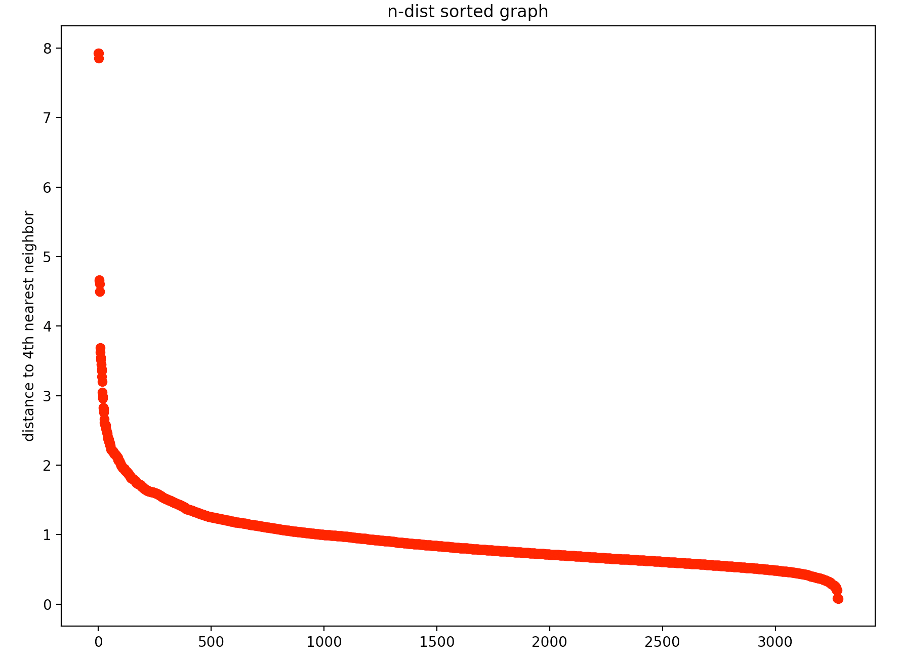
\includegraphics[width=0.5\textwidth]{./images/kDistGraphDBSCAN1h.png}
%   \caption{Sorted 4-dist graph of the 3h data set (distance for each point to its fourth nearest neighbor). The valley starts at roughly the 4th nearest neighbor distance of 2.}
%   \label{figure:kDistGraphDBSCAN1h}
% \end{figure*}

% \begin{figure*}[h]
%   \centering
%   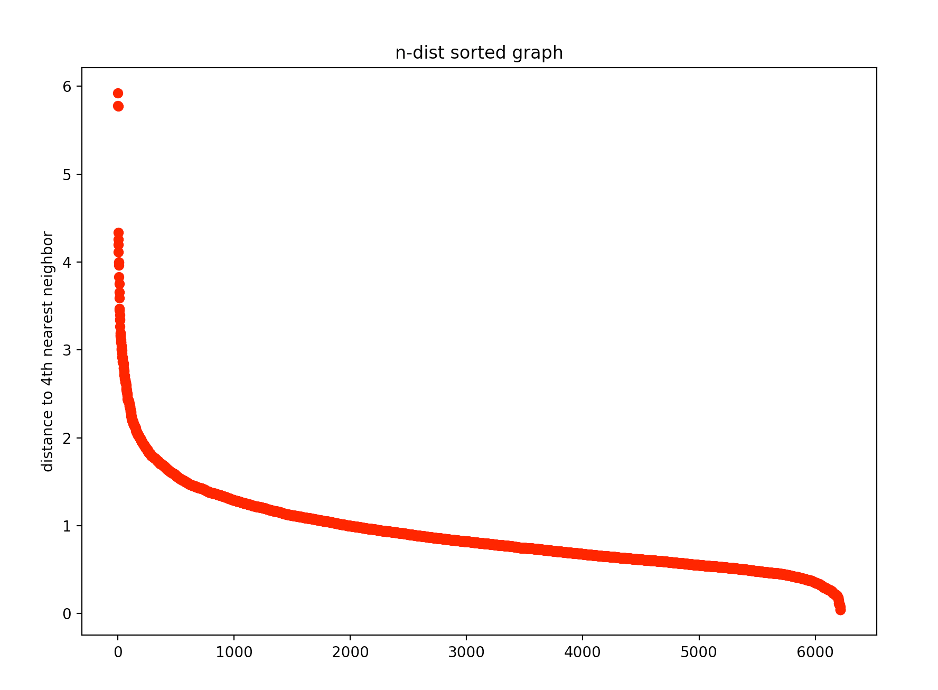
\includegraphics[width=0.5\textwidth]{./images/kDistGraphDBSCAN3h.png}
%   \caption{Sorted 4-dist graph of the 1h data set (distance for each point to its fourth nearest neighbor). The valley starts at roughly the 4th nearest neighbor distance of 2.}
%   \label{figure:kDistGraphDBSCAN3h}
% \end{figure*}


\begin{figure}[H]
  \centering
  \begin{subfigure}{.5\textwidth}
    \centering
    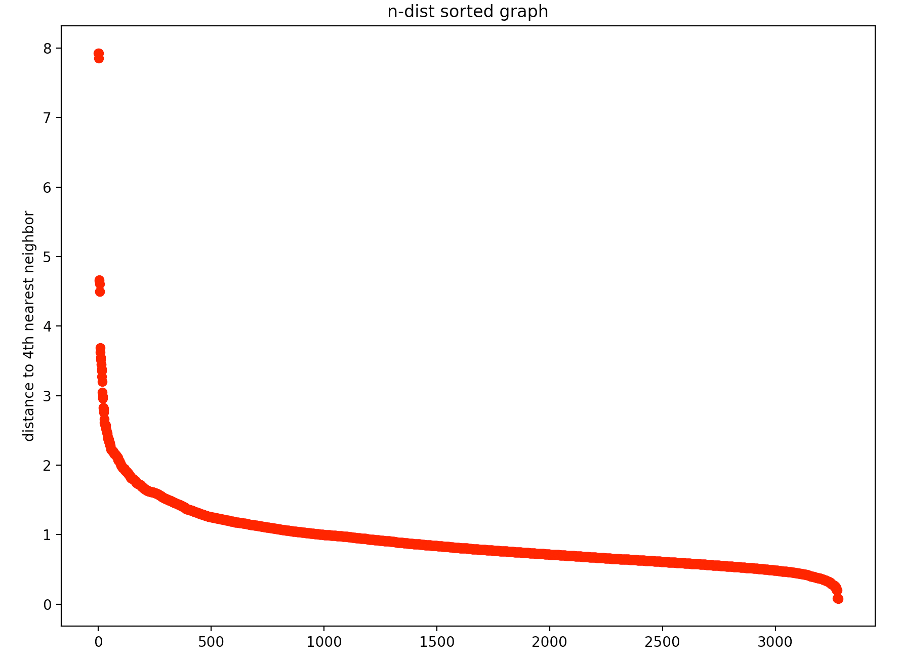
\includegraphics[width=0.87\textwidth]{./images/kDistGraphDBSCAN1h.png}
  \caption{1h data set}
  \label{figure:kDistGraphDBSCAN1h}
  \end{subfigure}%
  \begin{subfigure}{.5\textwidth}
    \centering
    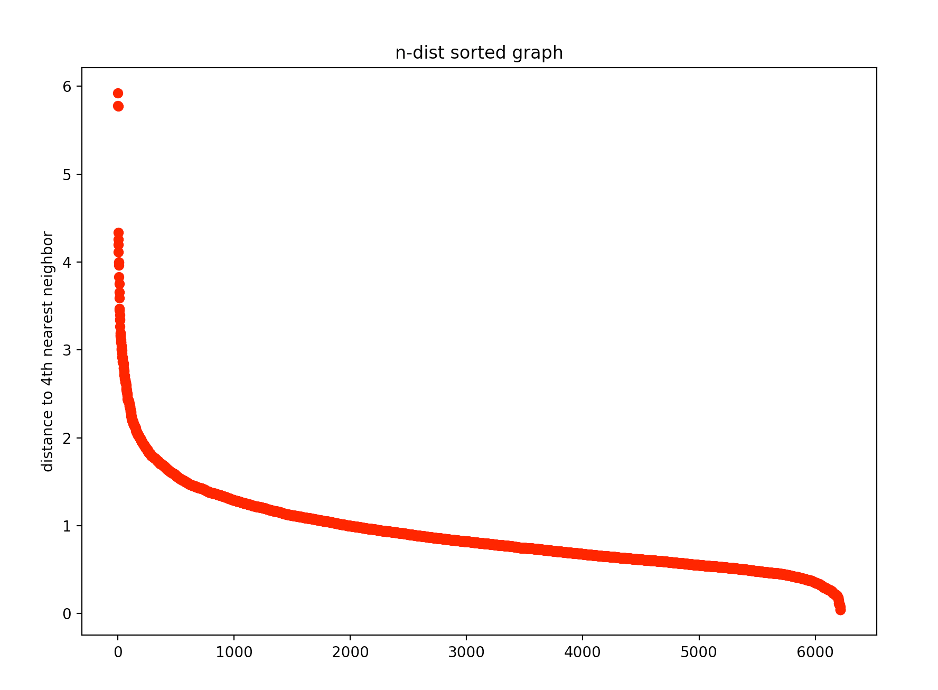
\includegraphics[width=1\textwidth]{./images/kDistGraphDBSCAN3h.png}
    \caption{3h data set}
    \label{figure:kDistGraphDBSCAN3h}
  \end{subfigure}
  \caption{Sorted 4-dist graphs (distance for each point to its fourth nearest neighbor), used to determine a suitable Eps parameter for the DBSCAN algorithm. The valley starts at roughly the 4th nearest neighbor distance of 2, therefore Eps should be 2.}
  \label{figure:kDistGraphDBSCAN}
  \end{figure}

The DBSCAN method was applied, with the parameters eps = 2 and min\_samples (MinPts) = 4. The results of this clustering method can be seen in figure \ref{figure:DBSCANResults}.


\begin{figure}[H]
  \centering
  \begin{subfigure}{.5\textwidth}
    \centering
    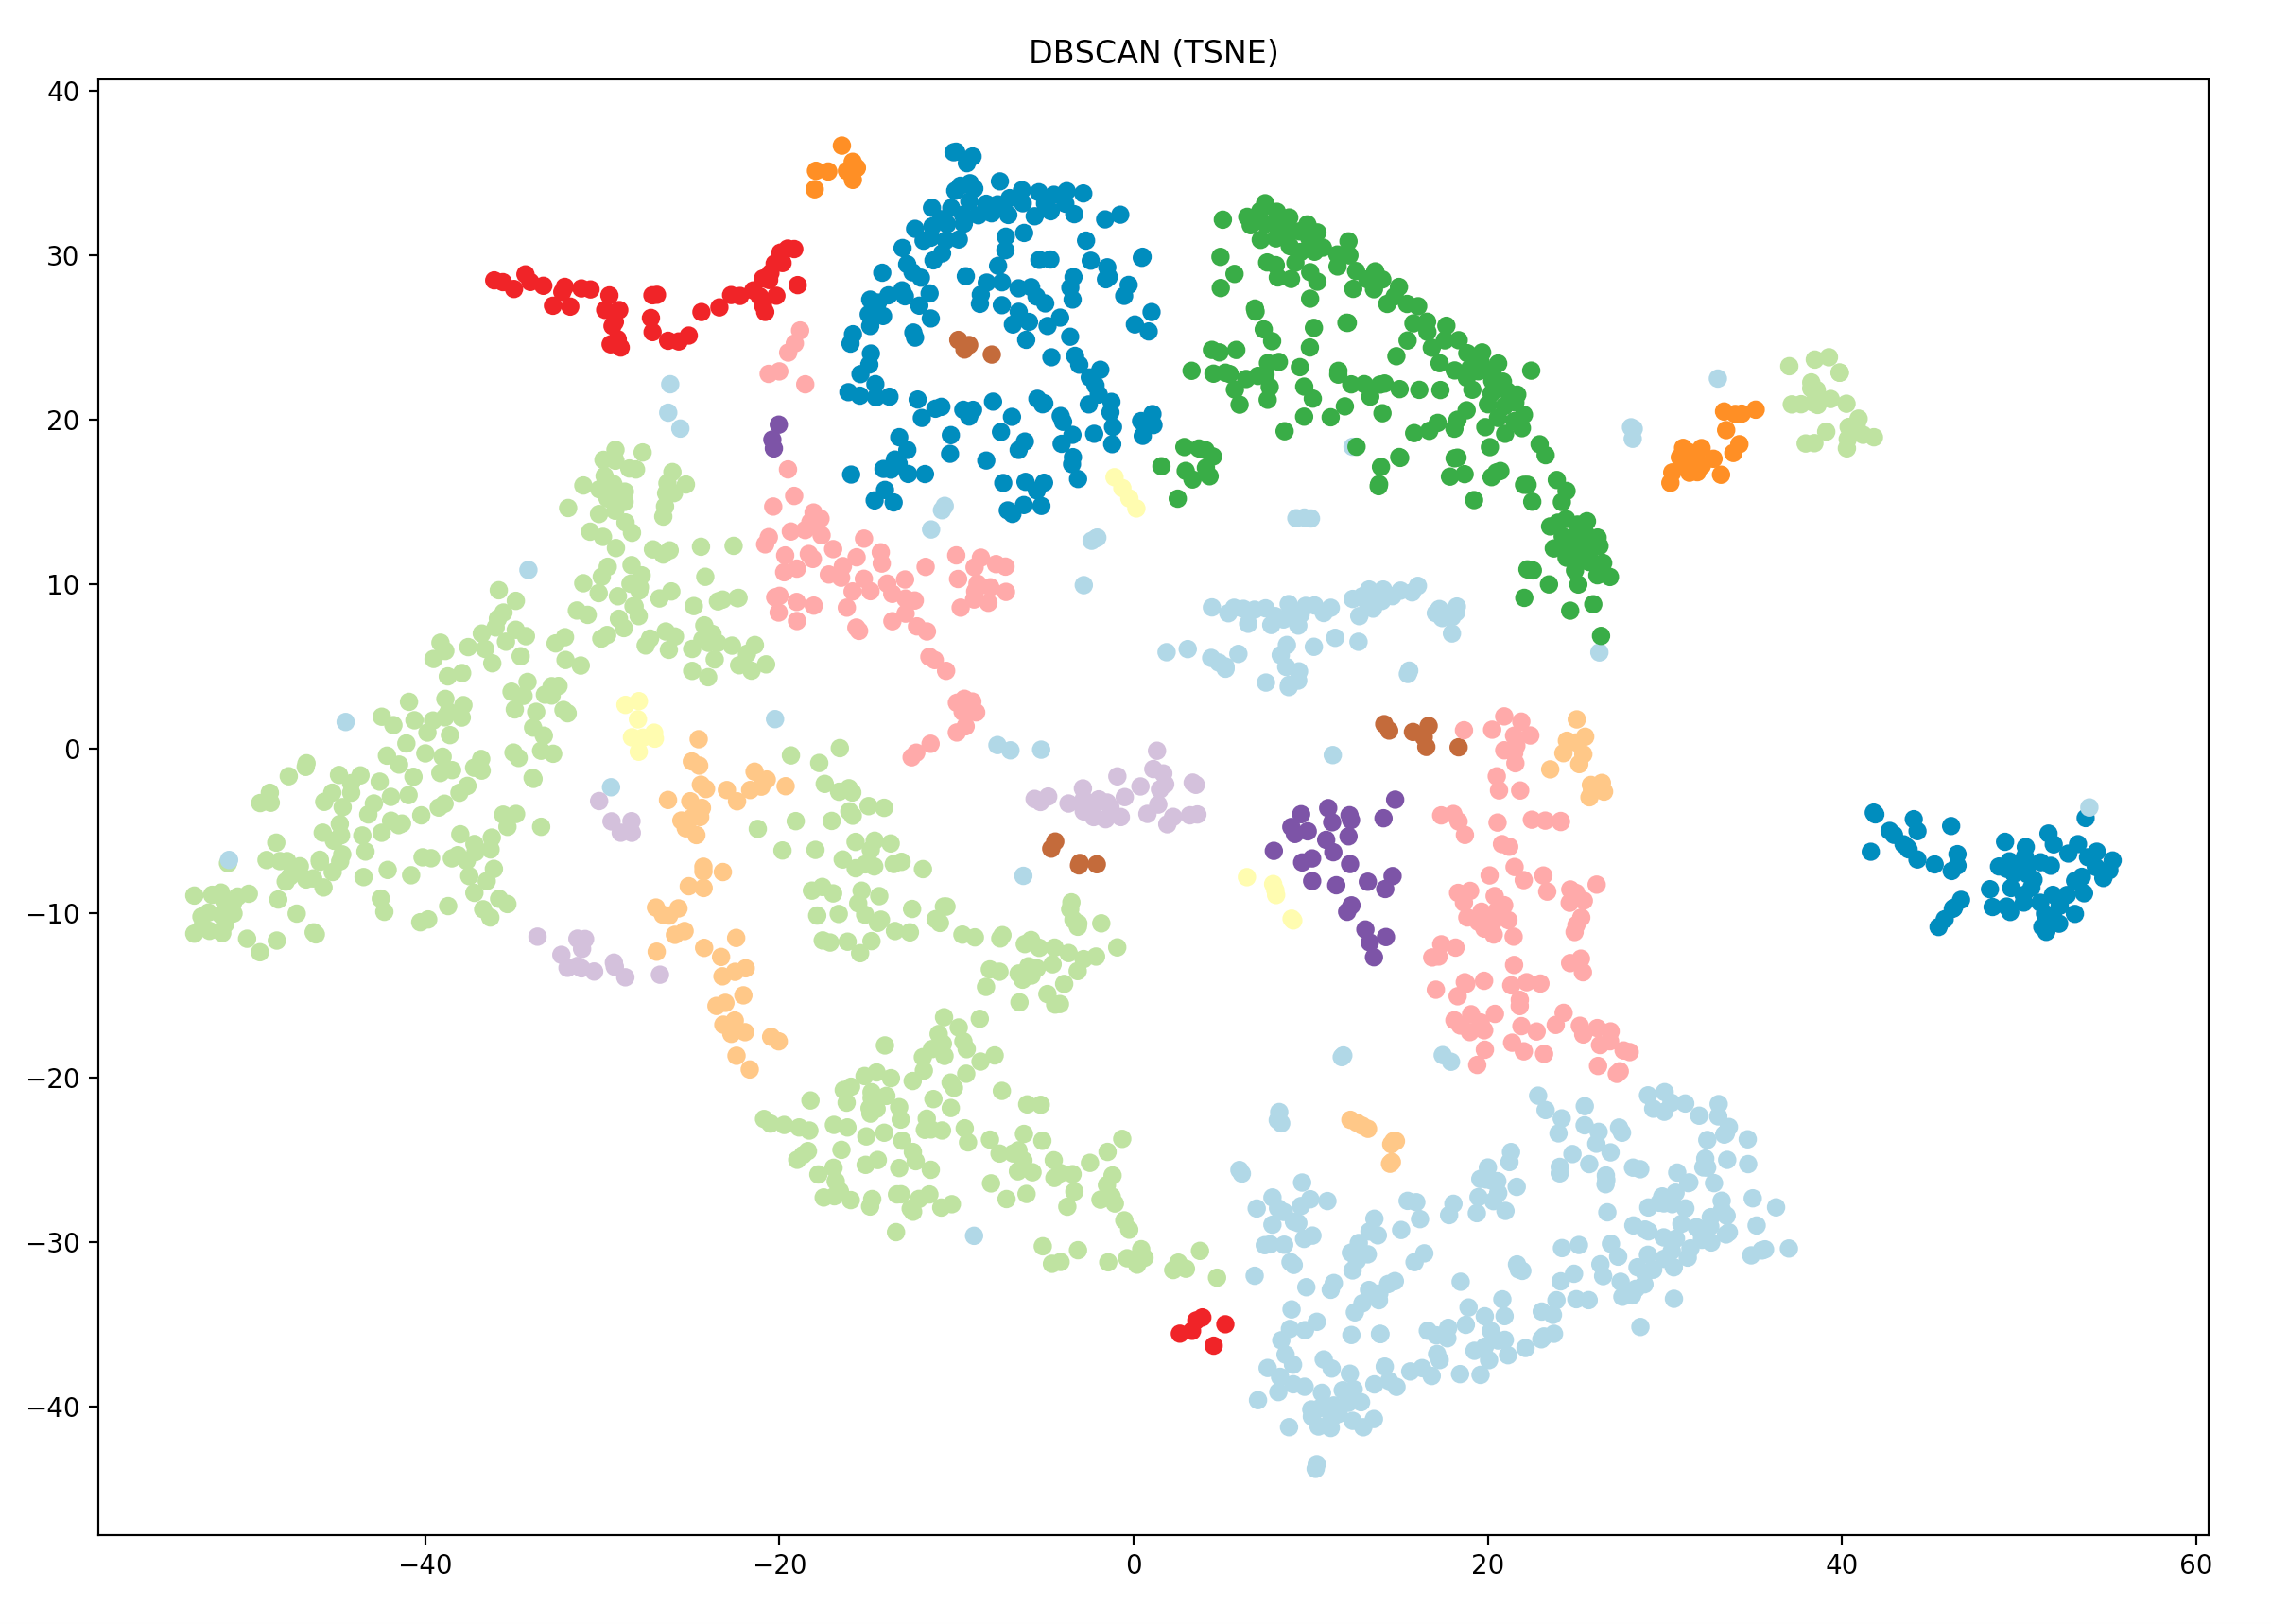
\includegraphics[width=1\textwidth]{./images/clusteringResults/1h-1-DBSCAN.png}
  \caption{1h data set DBSCAN clustering (first column - 15 min).}
  % \label{figure:1h-1-DBSCAN}
  \end{subfigure}%
  \begin{subfigure}{.5\textwidth}
    \centering
    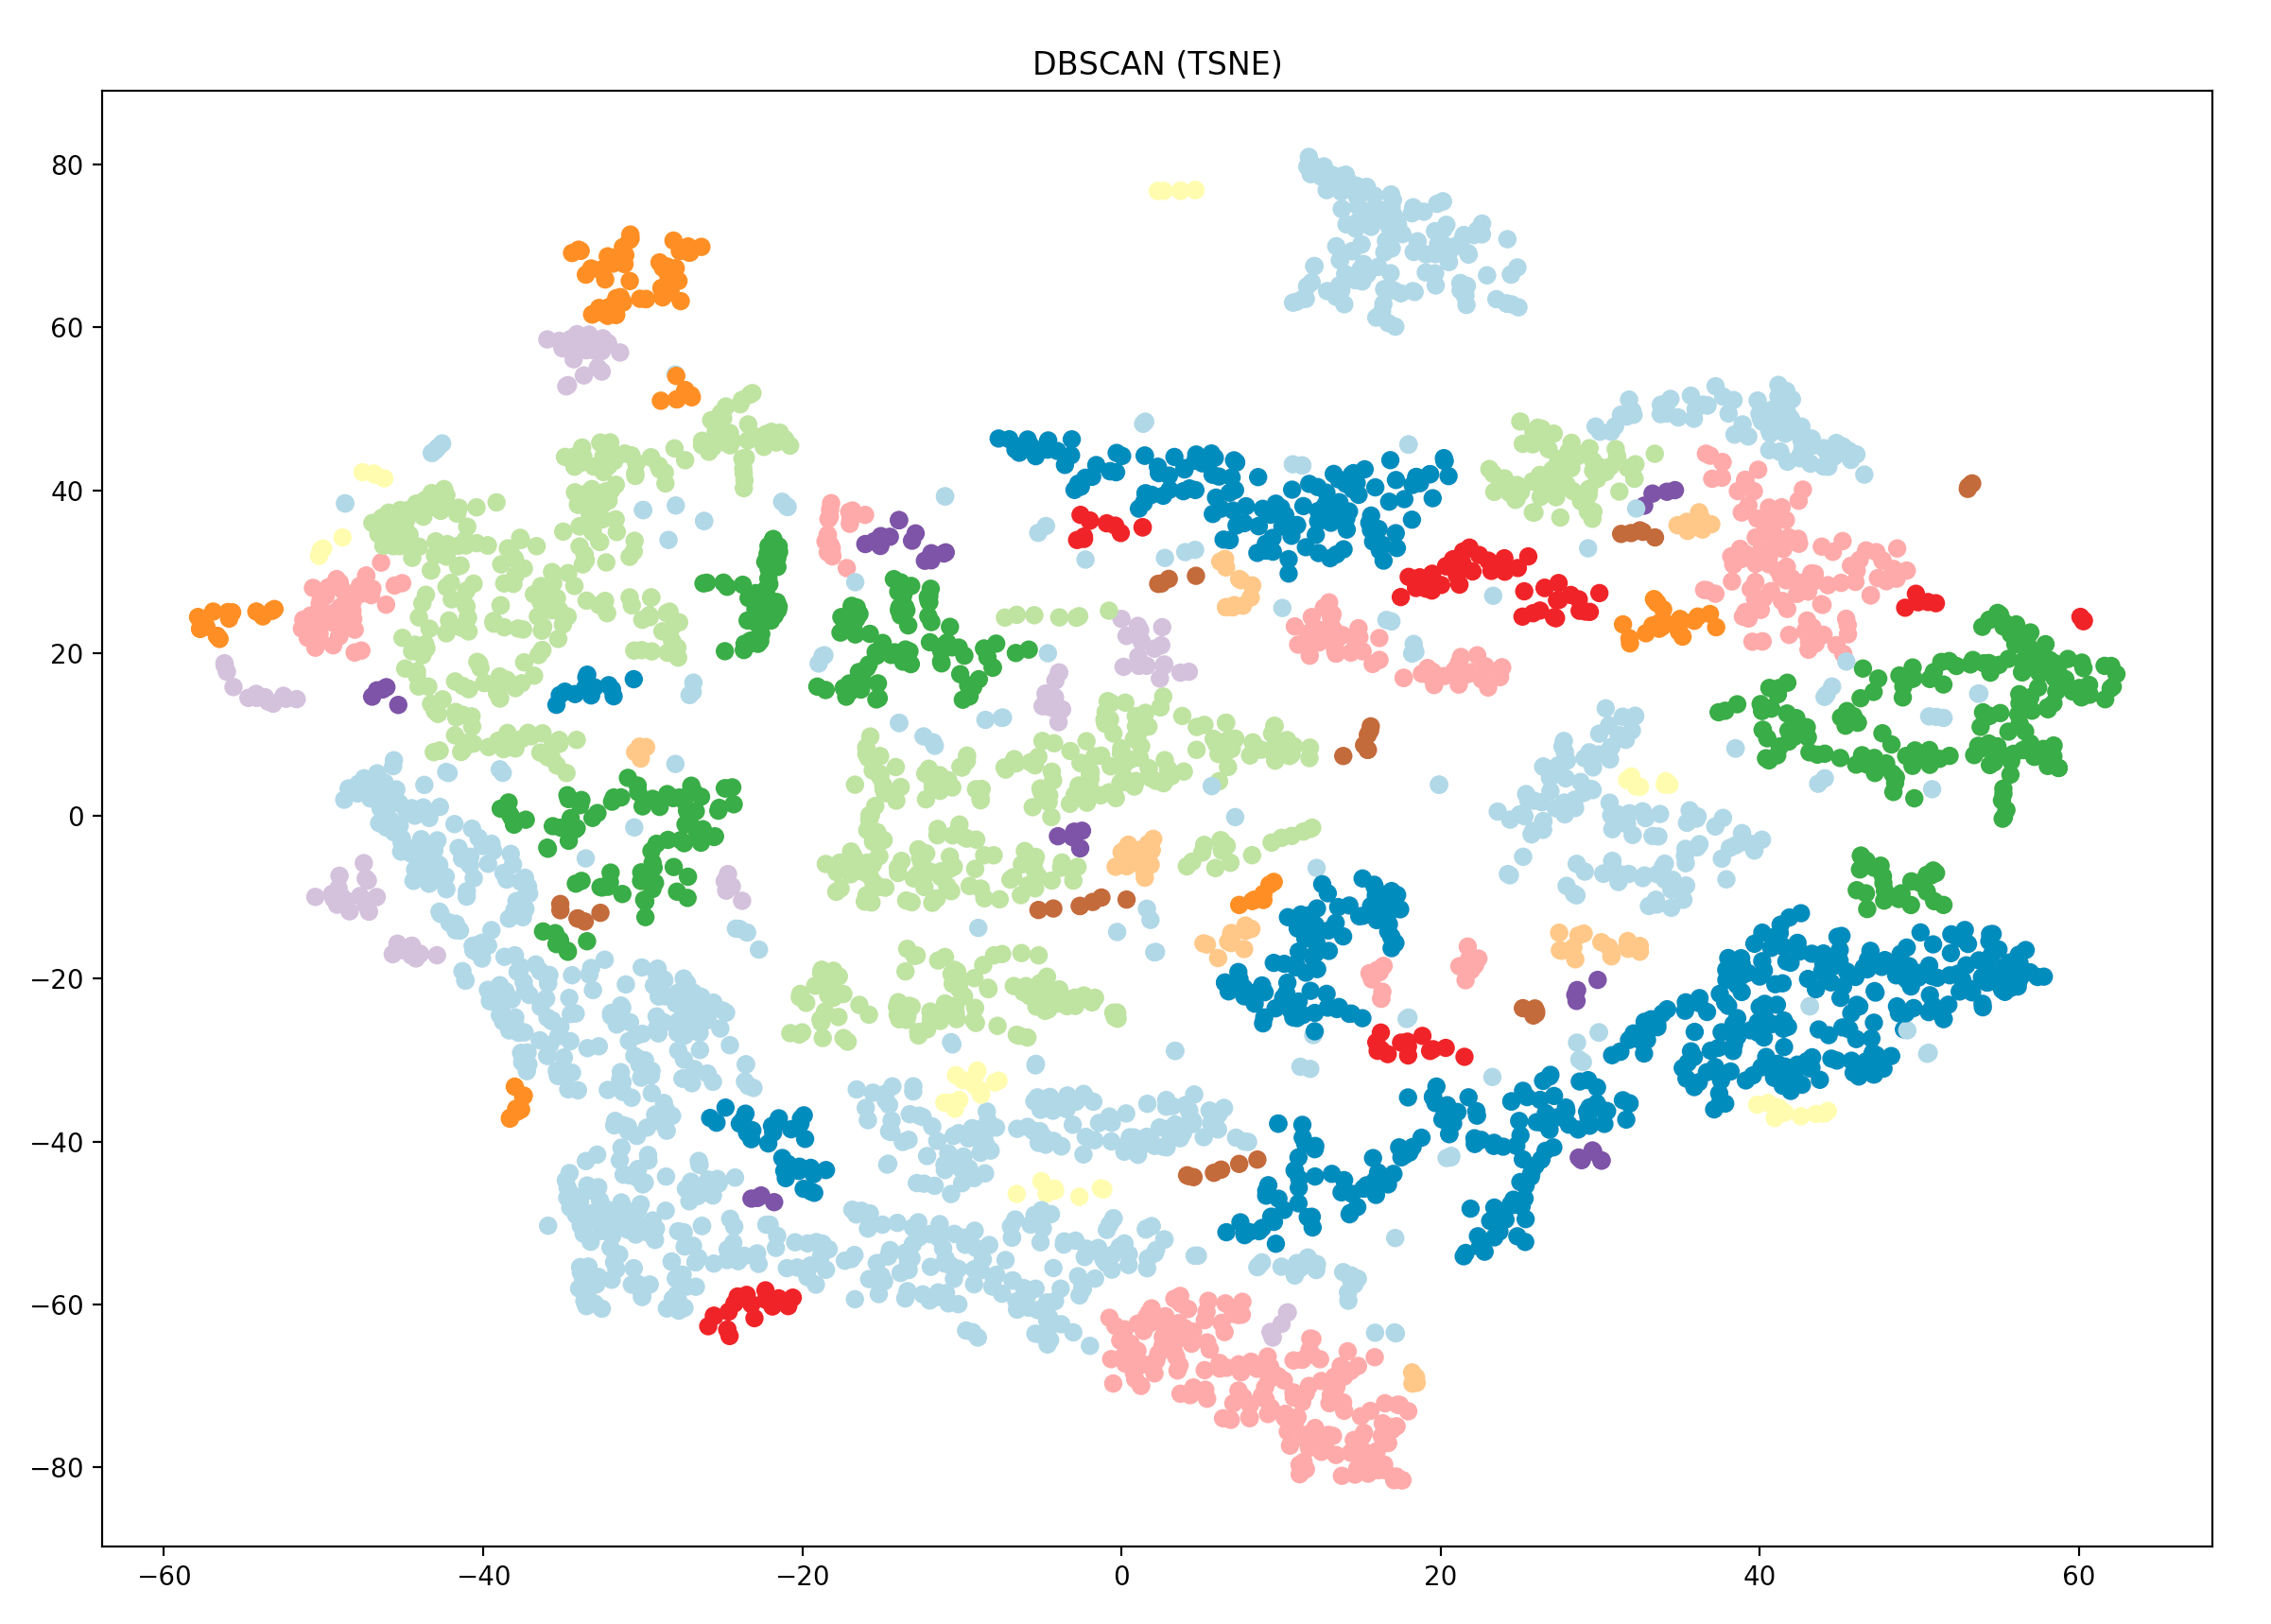
\includegraphics[width=1\textwidth]{./images/clusteringResults/3h-1-DBSCAN.png}
    \caption{3h data set DBSCAN clustering (first column - 30 min).}
    % \label{figure:3h-1-DBSCAN}
  \end{subfigure}
  \caption{}
  \label{figure:DBSCANResults}
  \end{figure}






\subsubsection{OPTICS}
The OPTICS algorithm was also implemented with its sklearn function\footnote{\url{https://scikit-learn.org/stable/modules/generated/sklearn.cluster.OPTICS.html}}. As stated in section \ref{section:OPTICS}, the OPTICS algorithm creates a reachability plot for the data points. The plots created for the SmartEater data files are depicted in \textbf{TODO FIGURES}. Initially, the clusters were extracted using the clustering method "xi". This is the automatic cluster extraction method, as explained in section \ref{section:OPTICS} and in \textcite{OPTICS}[57]. The visual results of these clusterings contained a lot of noise ??? \textbf{todo, show both xi and dbscan comparison, and explain why, also show silhouette, ... scores to prove that dbscan method provided better clusters}
\textbf{todo: see reachability plots full size in appendix}
\textbf{todo: convert reachability plot to bar chart}

\begin{figure}[H]
  \centering
  \begin{subfigure}{.5\textwidth}
    \centering
    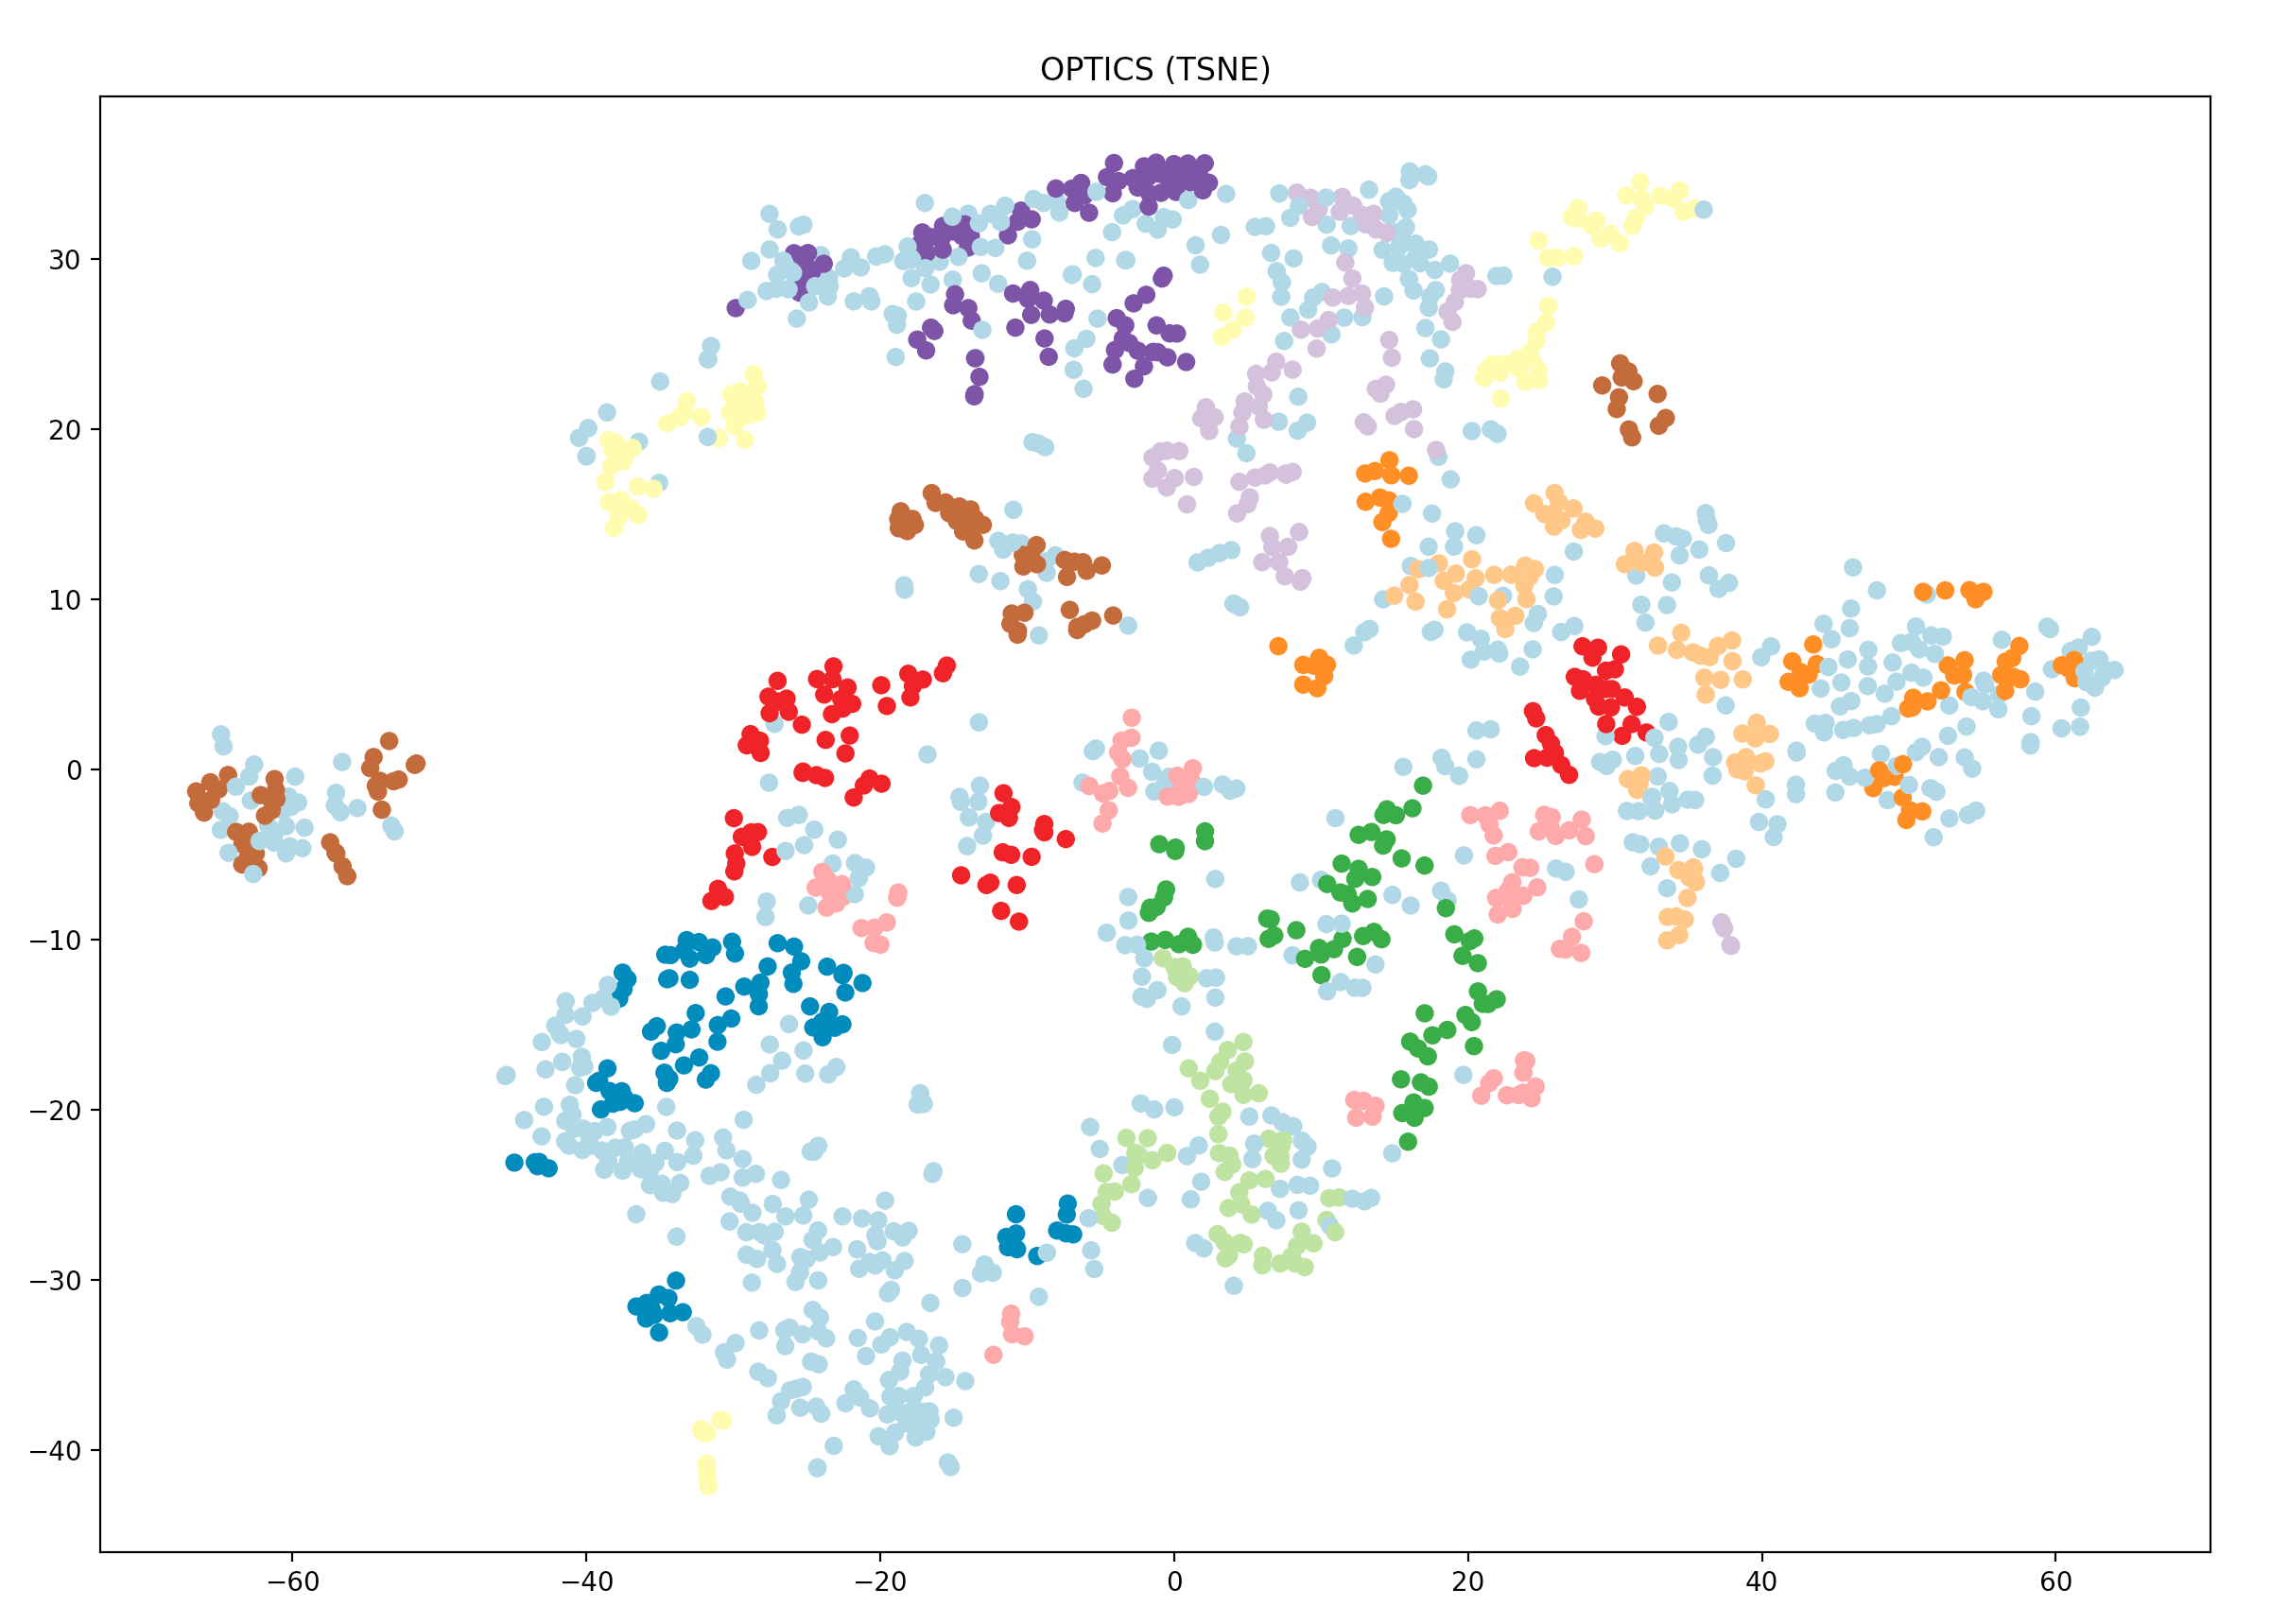
\includegraphics[width=1\textwidth]{./images/clusteringResults/1h-1-OPTICS-xi.png}
  \caption{1h data set OPTICS clustering (first column - 30 min), using OPTICS automatic cluster extraction (xi).}
  % \label{figure:1h-1-OPTICS}
  \end{subfigure}%
  \begin{subfigure}{.5\textwidth}
    \centering
    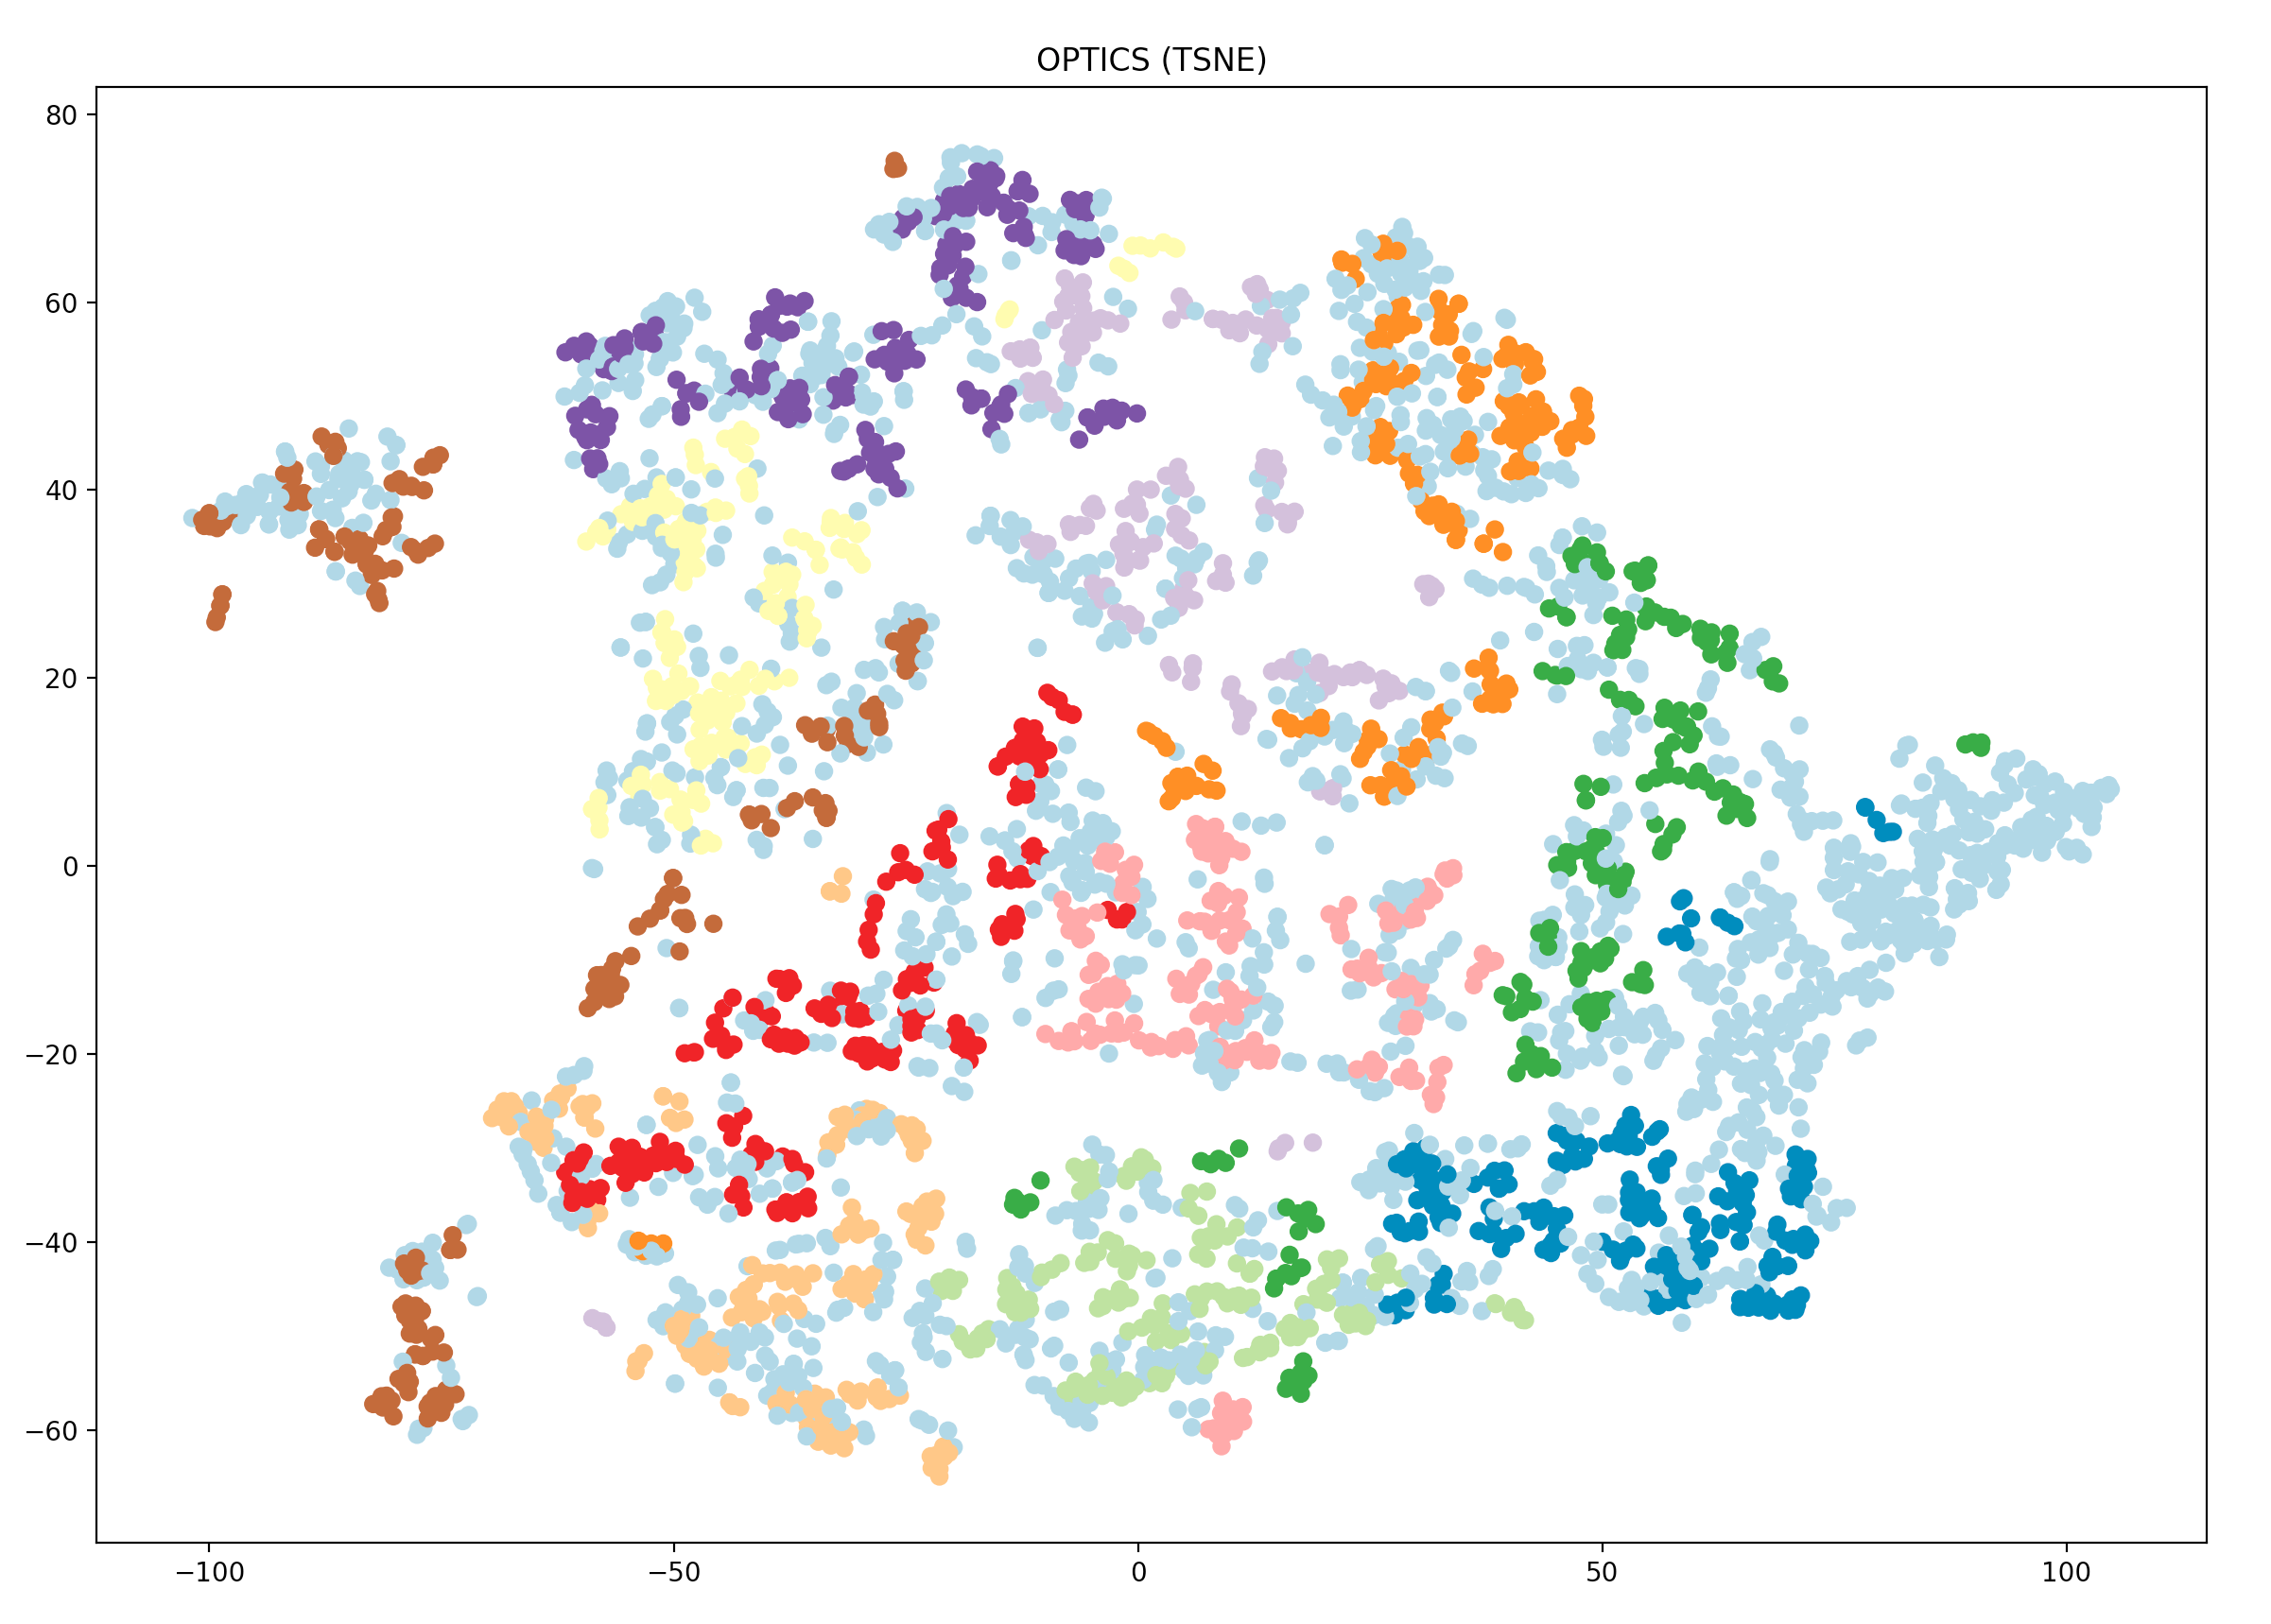
\includegraphics[width=1\textwidth]{./images/clusteringResults/3h-1-OPTICS-xi.png}
    \caption{3h data set OPTICS clustering (first column - 30 min), using OPTICS automatic cluster extraction (xi).}
    % \label{figure:3h-1-OPTICS}
  \end{subfigure}
  \caption{}
  \label{figure:OPTICSXiResults}
  \end{figure}

  \begin{figure}[H]
    \centering
    \begin{subfigure}{.5\textwidth}
      \centering
      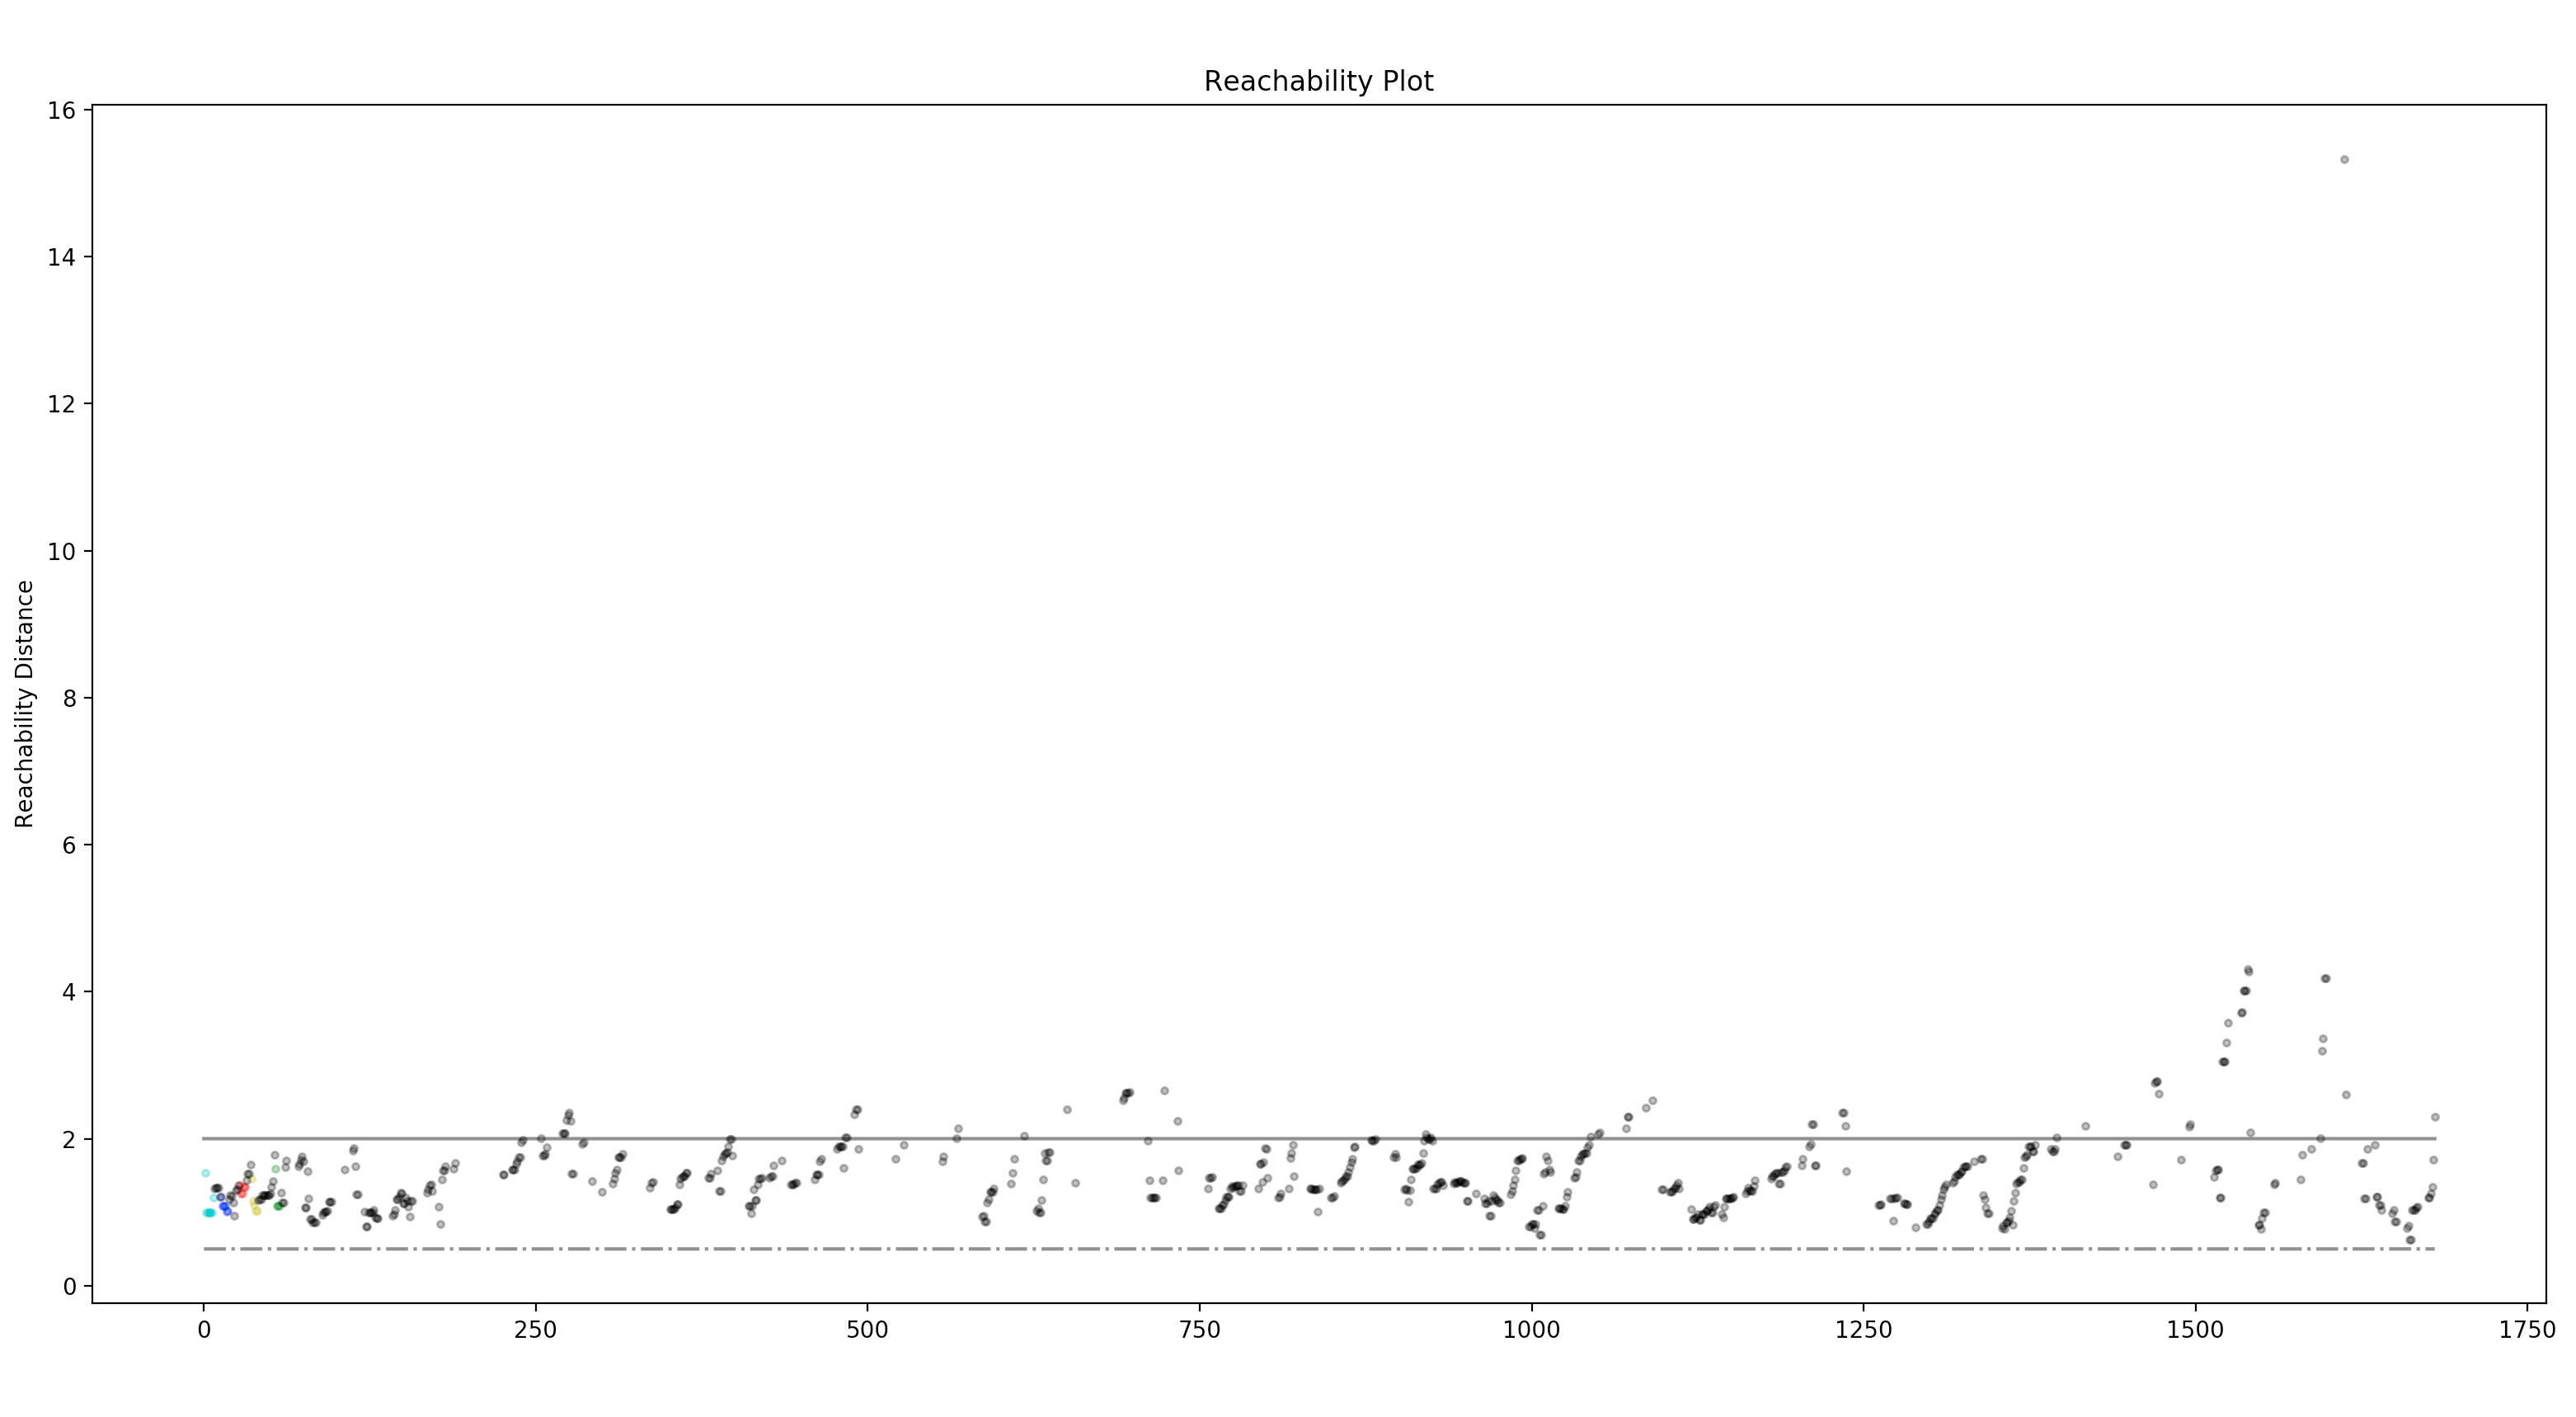
\includegraphics[width=1\textwidth]{./images/clusteringResults/1h-1-reachabilityPlot-xi.png}
    \caption{1h data set OPTICS clustering (first column - 15 min), using OPTICS automatic cluster extraction (xi).}
    % \label{figure:1h-1-reachabilityPlot}
    \end{subfigure}%
    \begin{subfigure}{.5\textwidth}
      \centering
      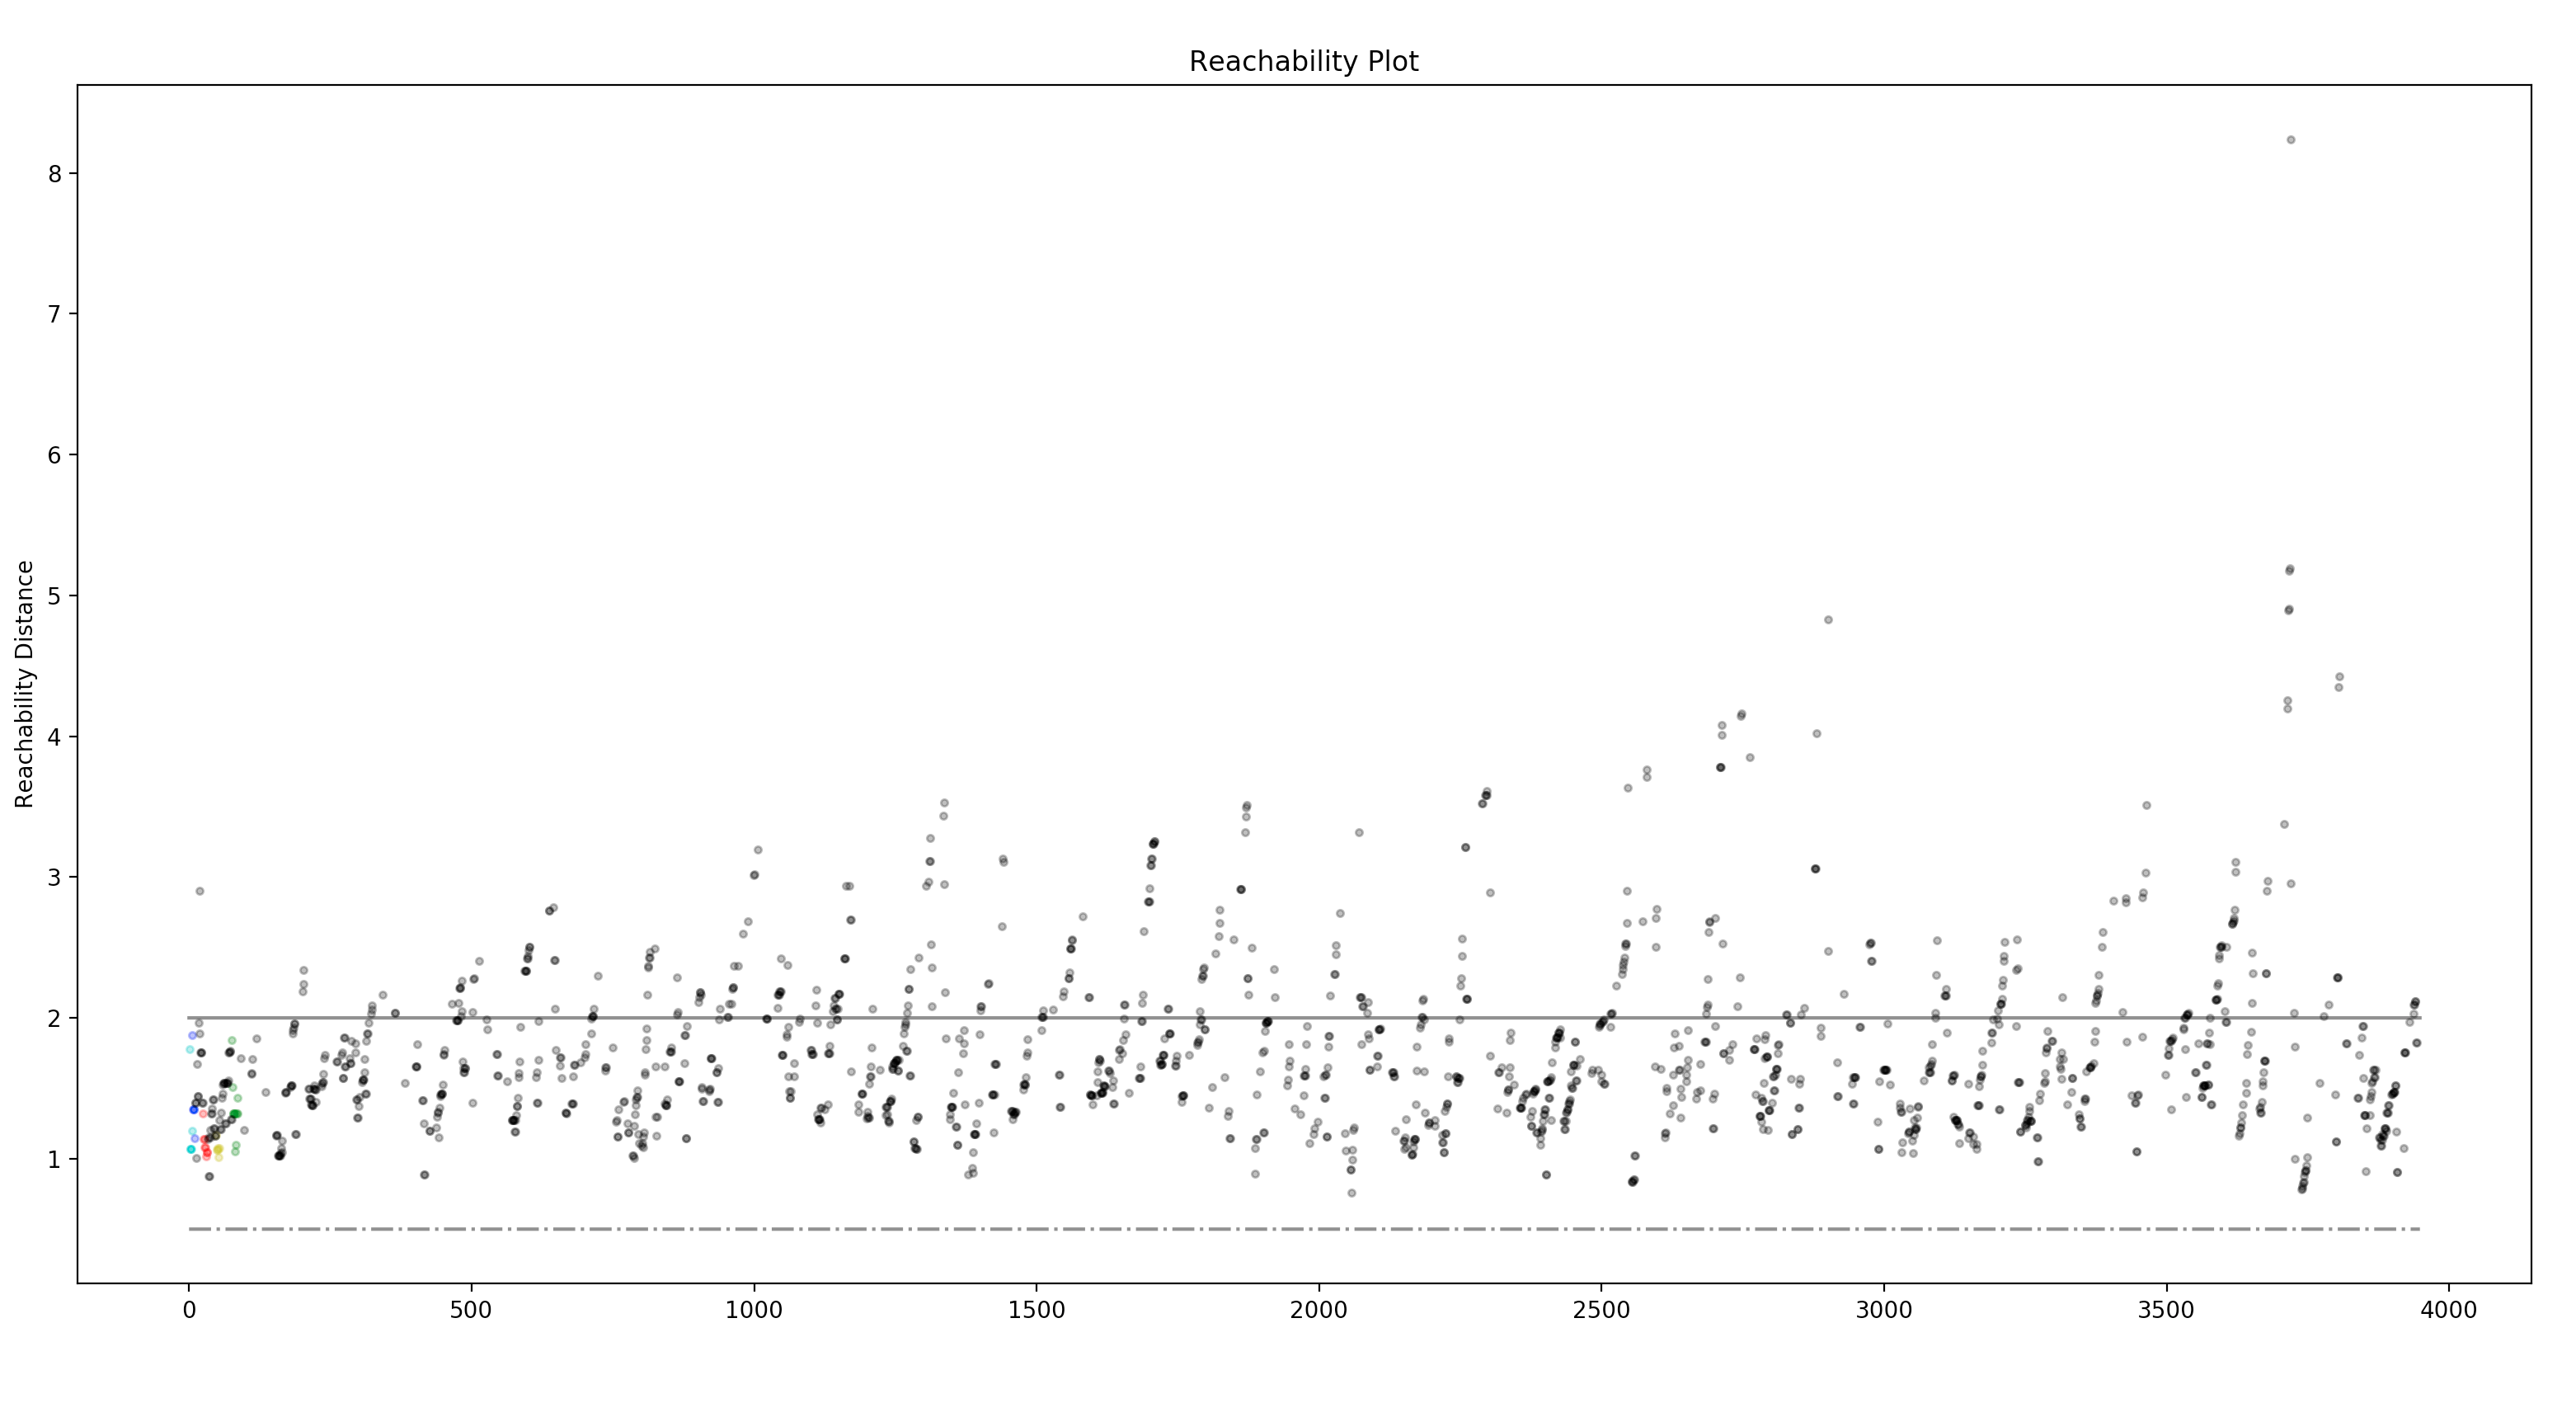
\includegraphics[width=1\textwidth]{./images/clusteringResults/3h-1-reachabilityPlot-xi.png}
      \caption{3h data set OPTICS clustering (first column - 30 min), using OPTICS automatic cluster extraction (xi).}
      % \label{figure:3h-1-reachabilityPlot}
    \end{subfigure}
    \caption{}
    \label{figure:OPTICSResultsReachabilityPlot}
    \end{figure}

\begin{figure}[H]
  \centering
  \begin{subfigure}{.5\textwidth}
    \centering
    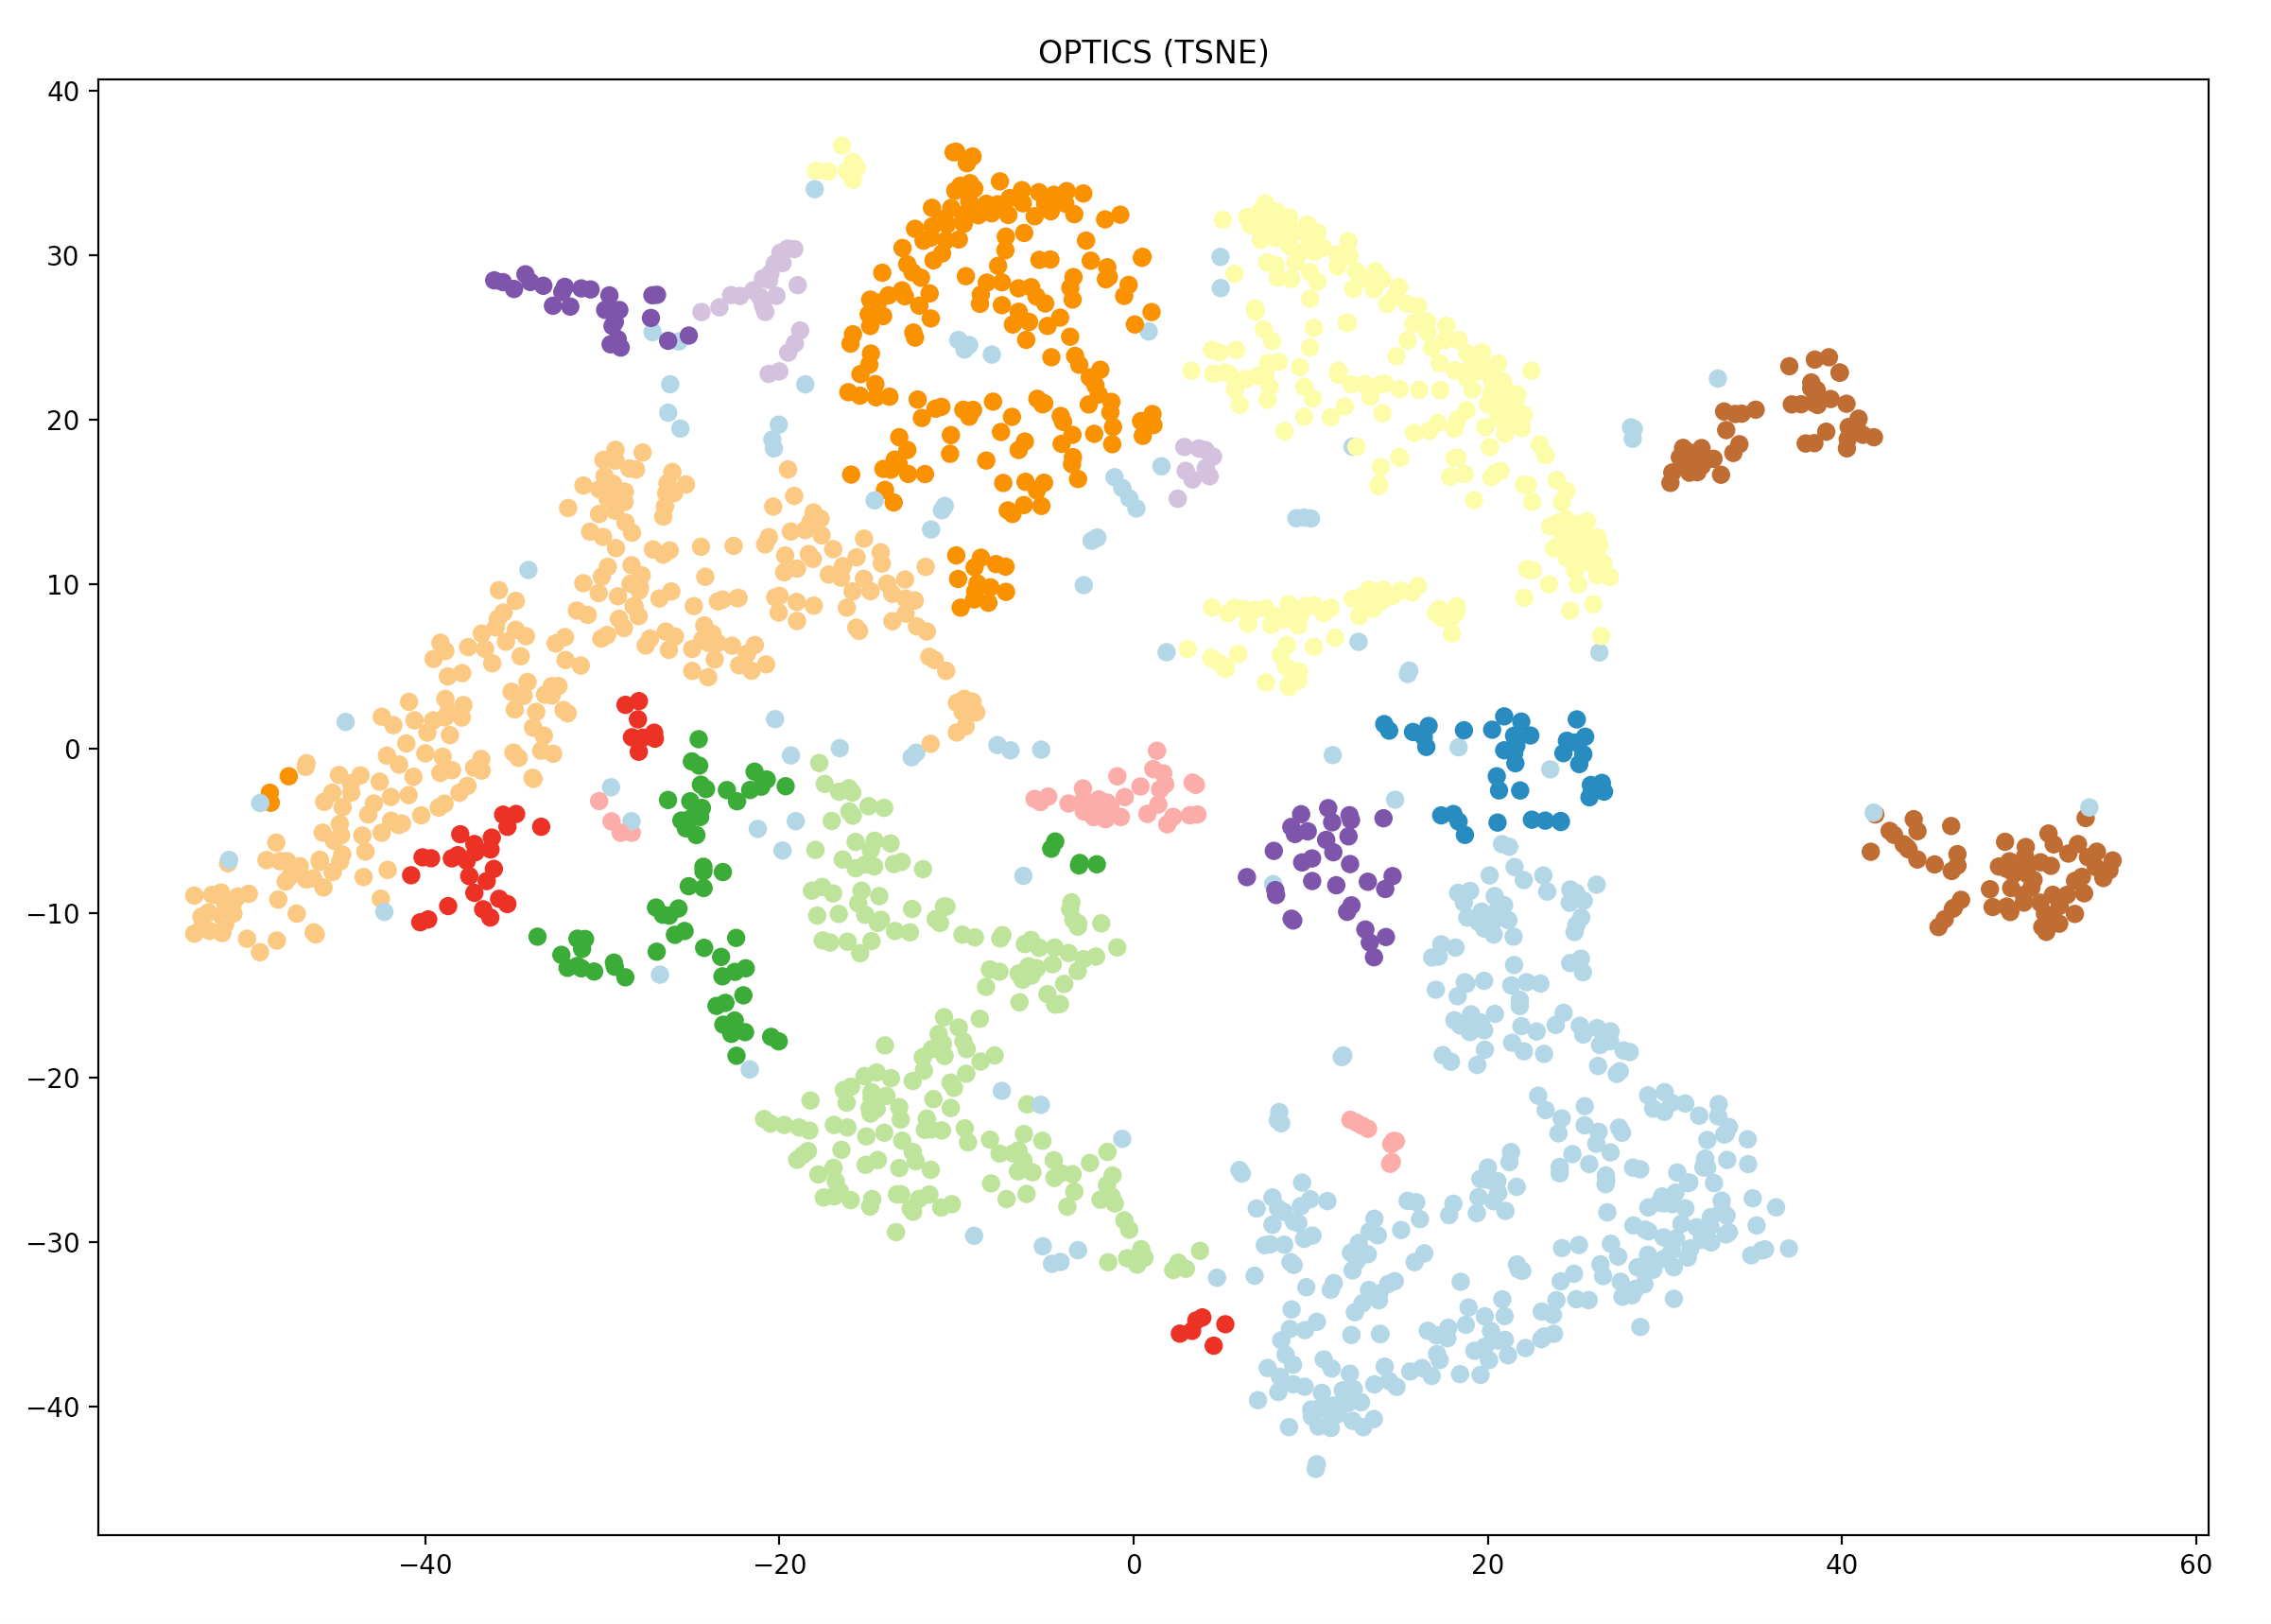
\includegraphics[width=1\textwidth]{./images/clusteringResults/1h-1-OPTICS.png}
  \caption{1h data set OPTICS clustering (first column - 15 min), using DBSCAN clustering.}
  % \label{figure:1h-1-OPTICS}
  \end{subfigure}%
  \begin{subfigure}{.5\textwidth}
    \centering
    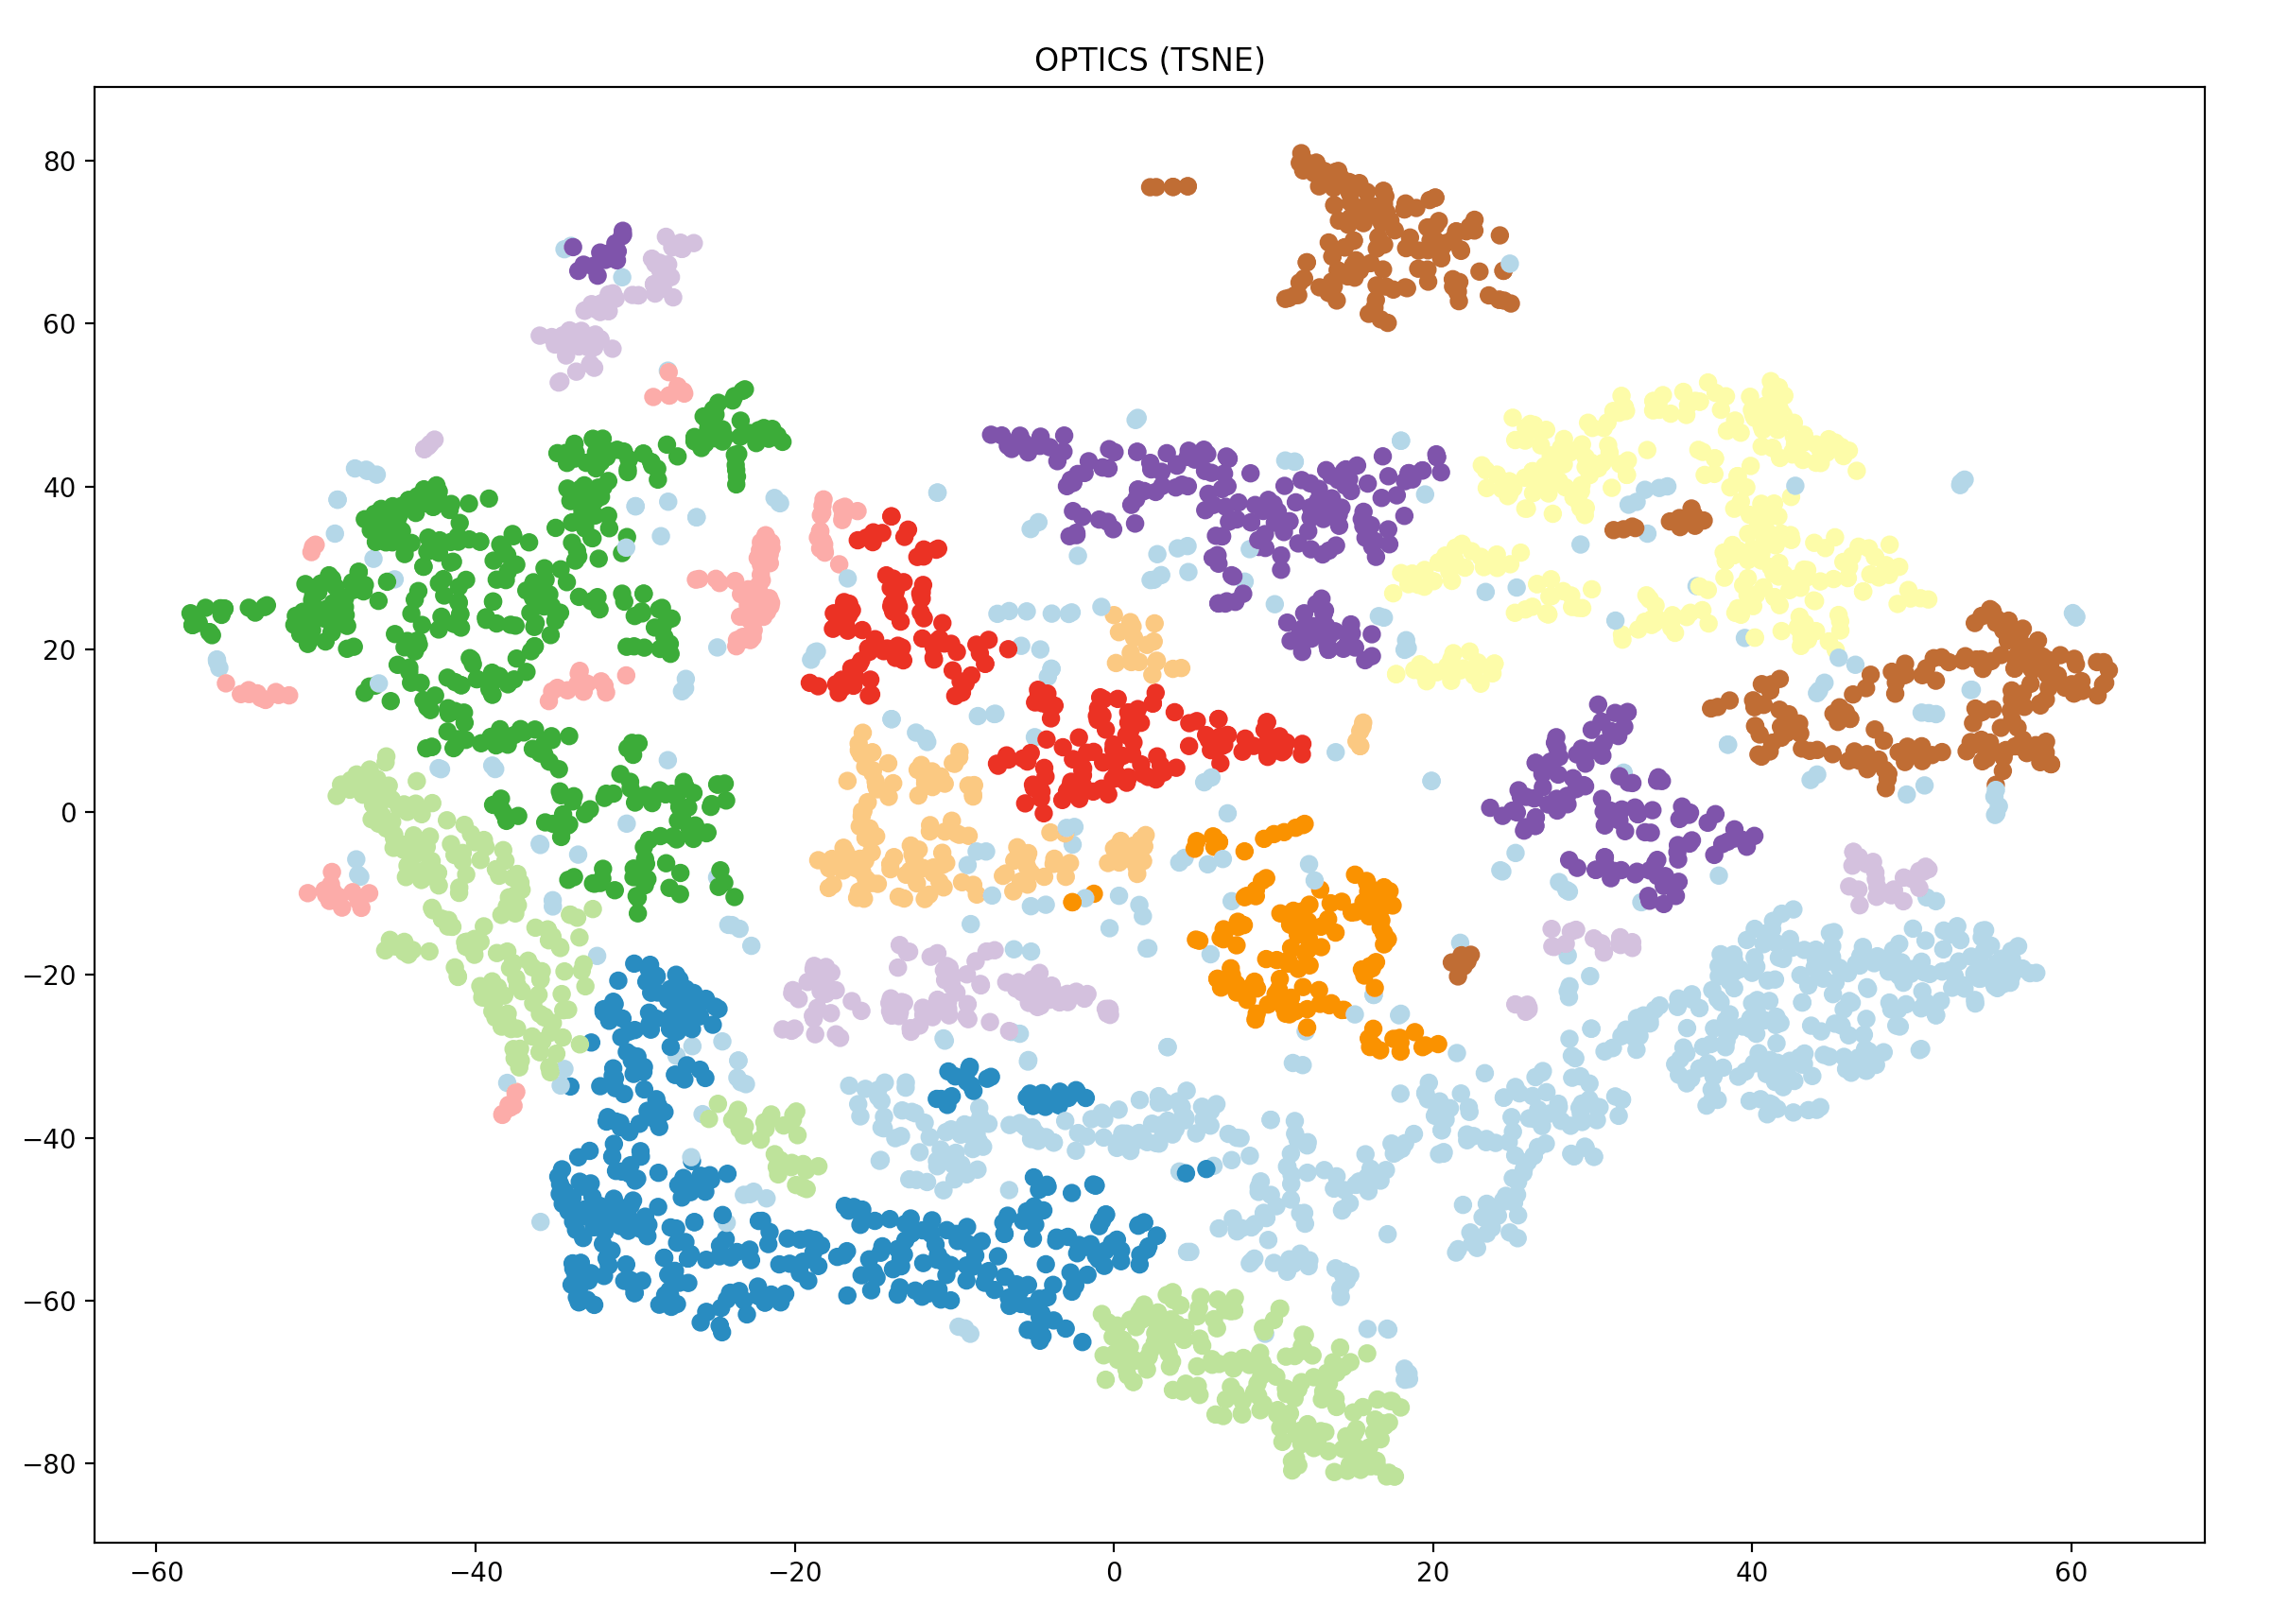
\includegraphics[width=1\textwidth]{./images/clusteringResults/3h-1-OPTICS.png}
    \caption{3h data set OPTICS clustering (first column - 30 min), using DBSCAN clustering.}
    % \label{figure:3h-1-OPTICS}
  \end{subfigure}
  \caption{}
  \label{figure:OPTICSResults}
  \end{figure}

\begin{figure}[H]
  \centering
  \begin{subfigure}{.5\textwidth}
    \centering
    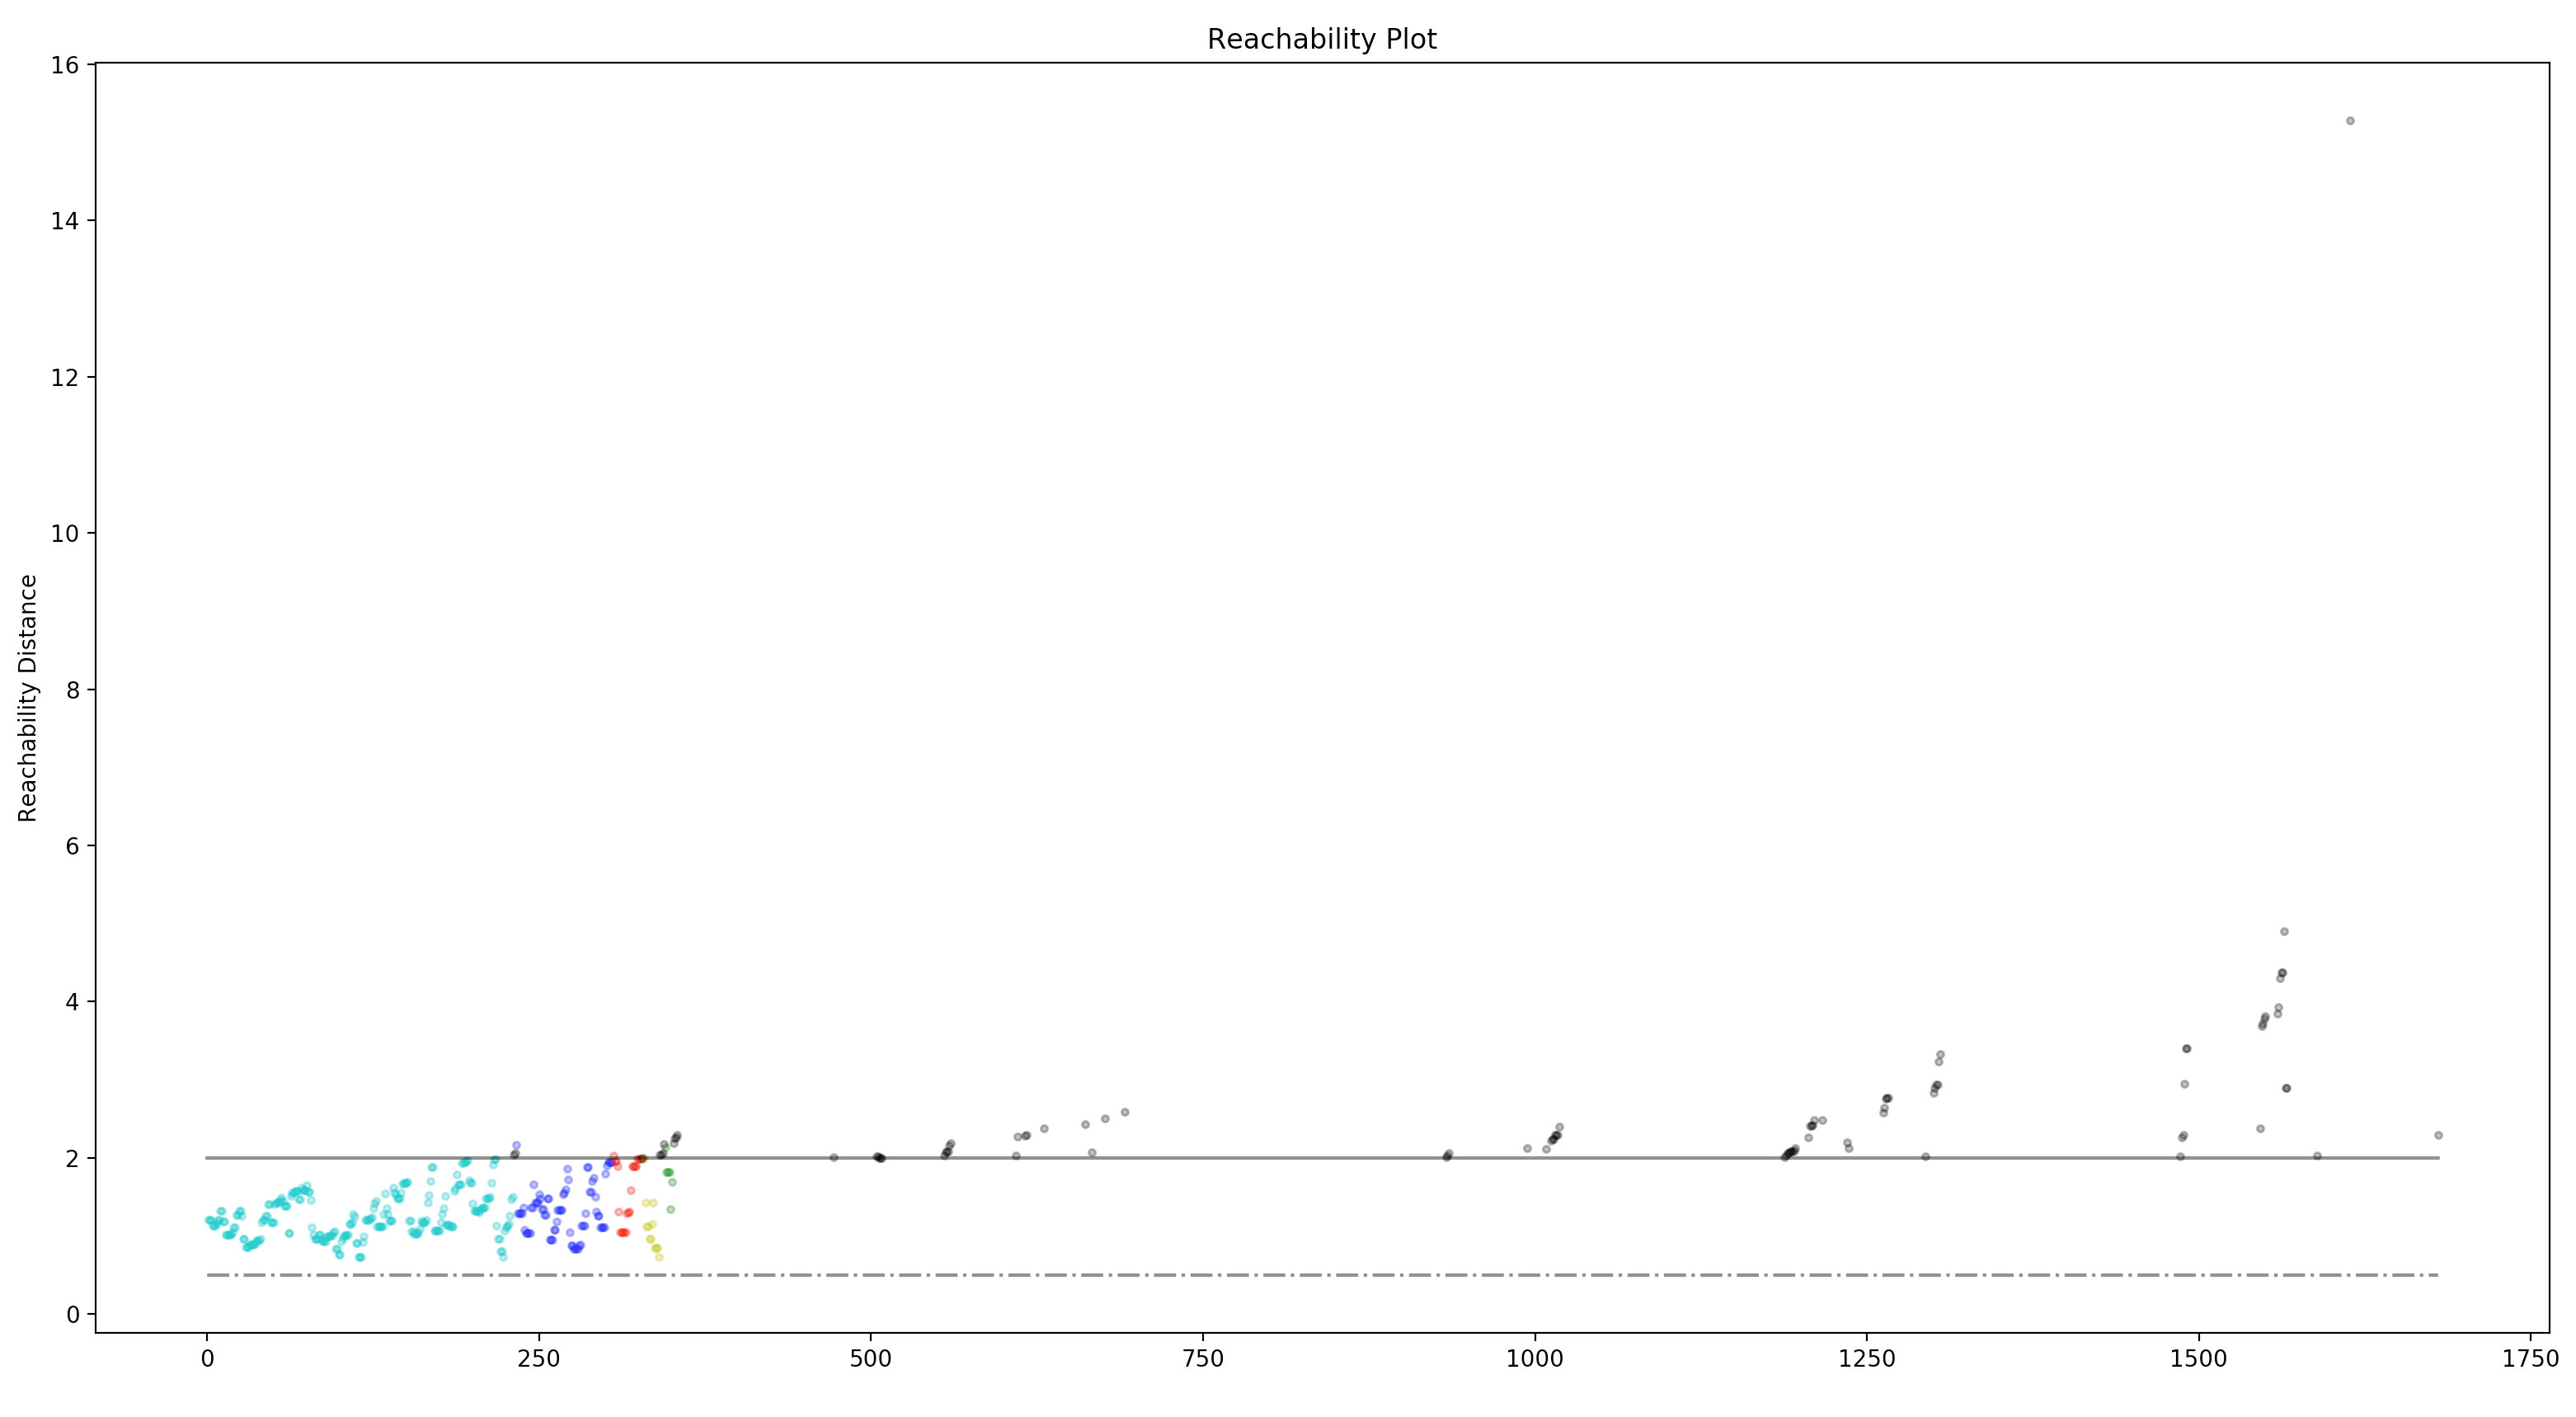
\includegraphics[width=1\textwidth]{./images/clusteringResults/1h-1-reachabilityPlot.png}
  \caption{1h data set OPTICS clustering (first column - 15 min), using DBSCAN clustering.}
  % \label{figure:1h-1-reachabilityPlot}
  \end{subfigure}%
  \begin{subfigure}{.5\textwidth}
    \centering
    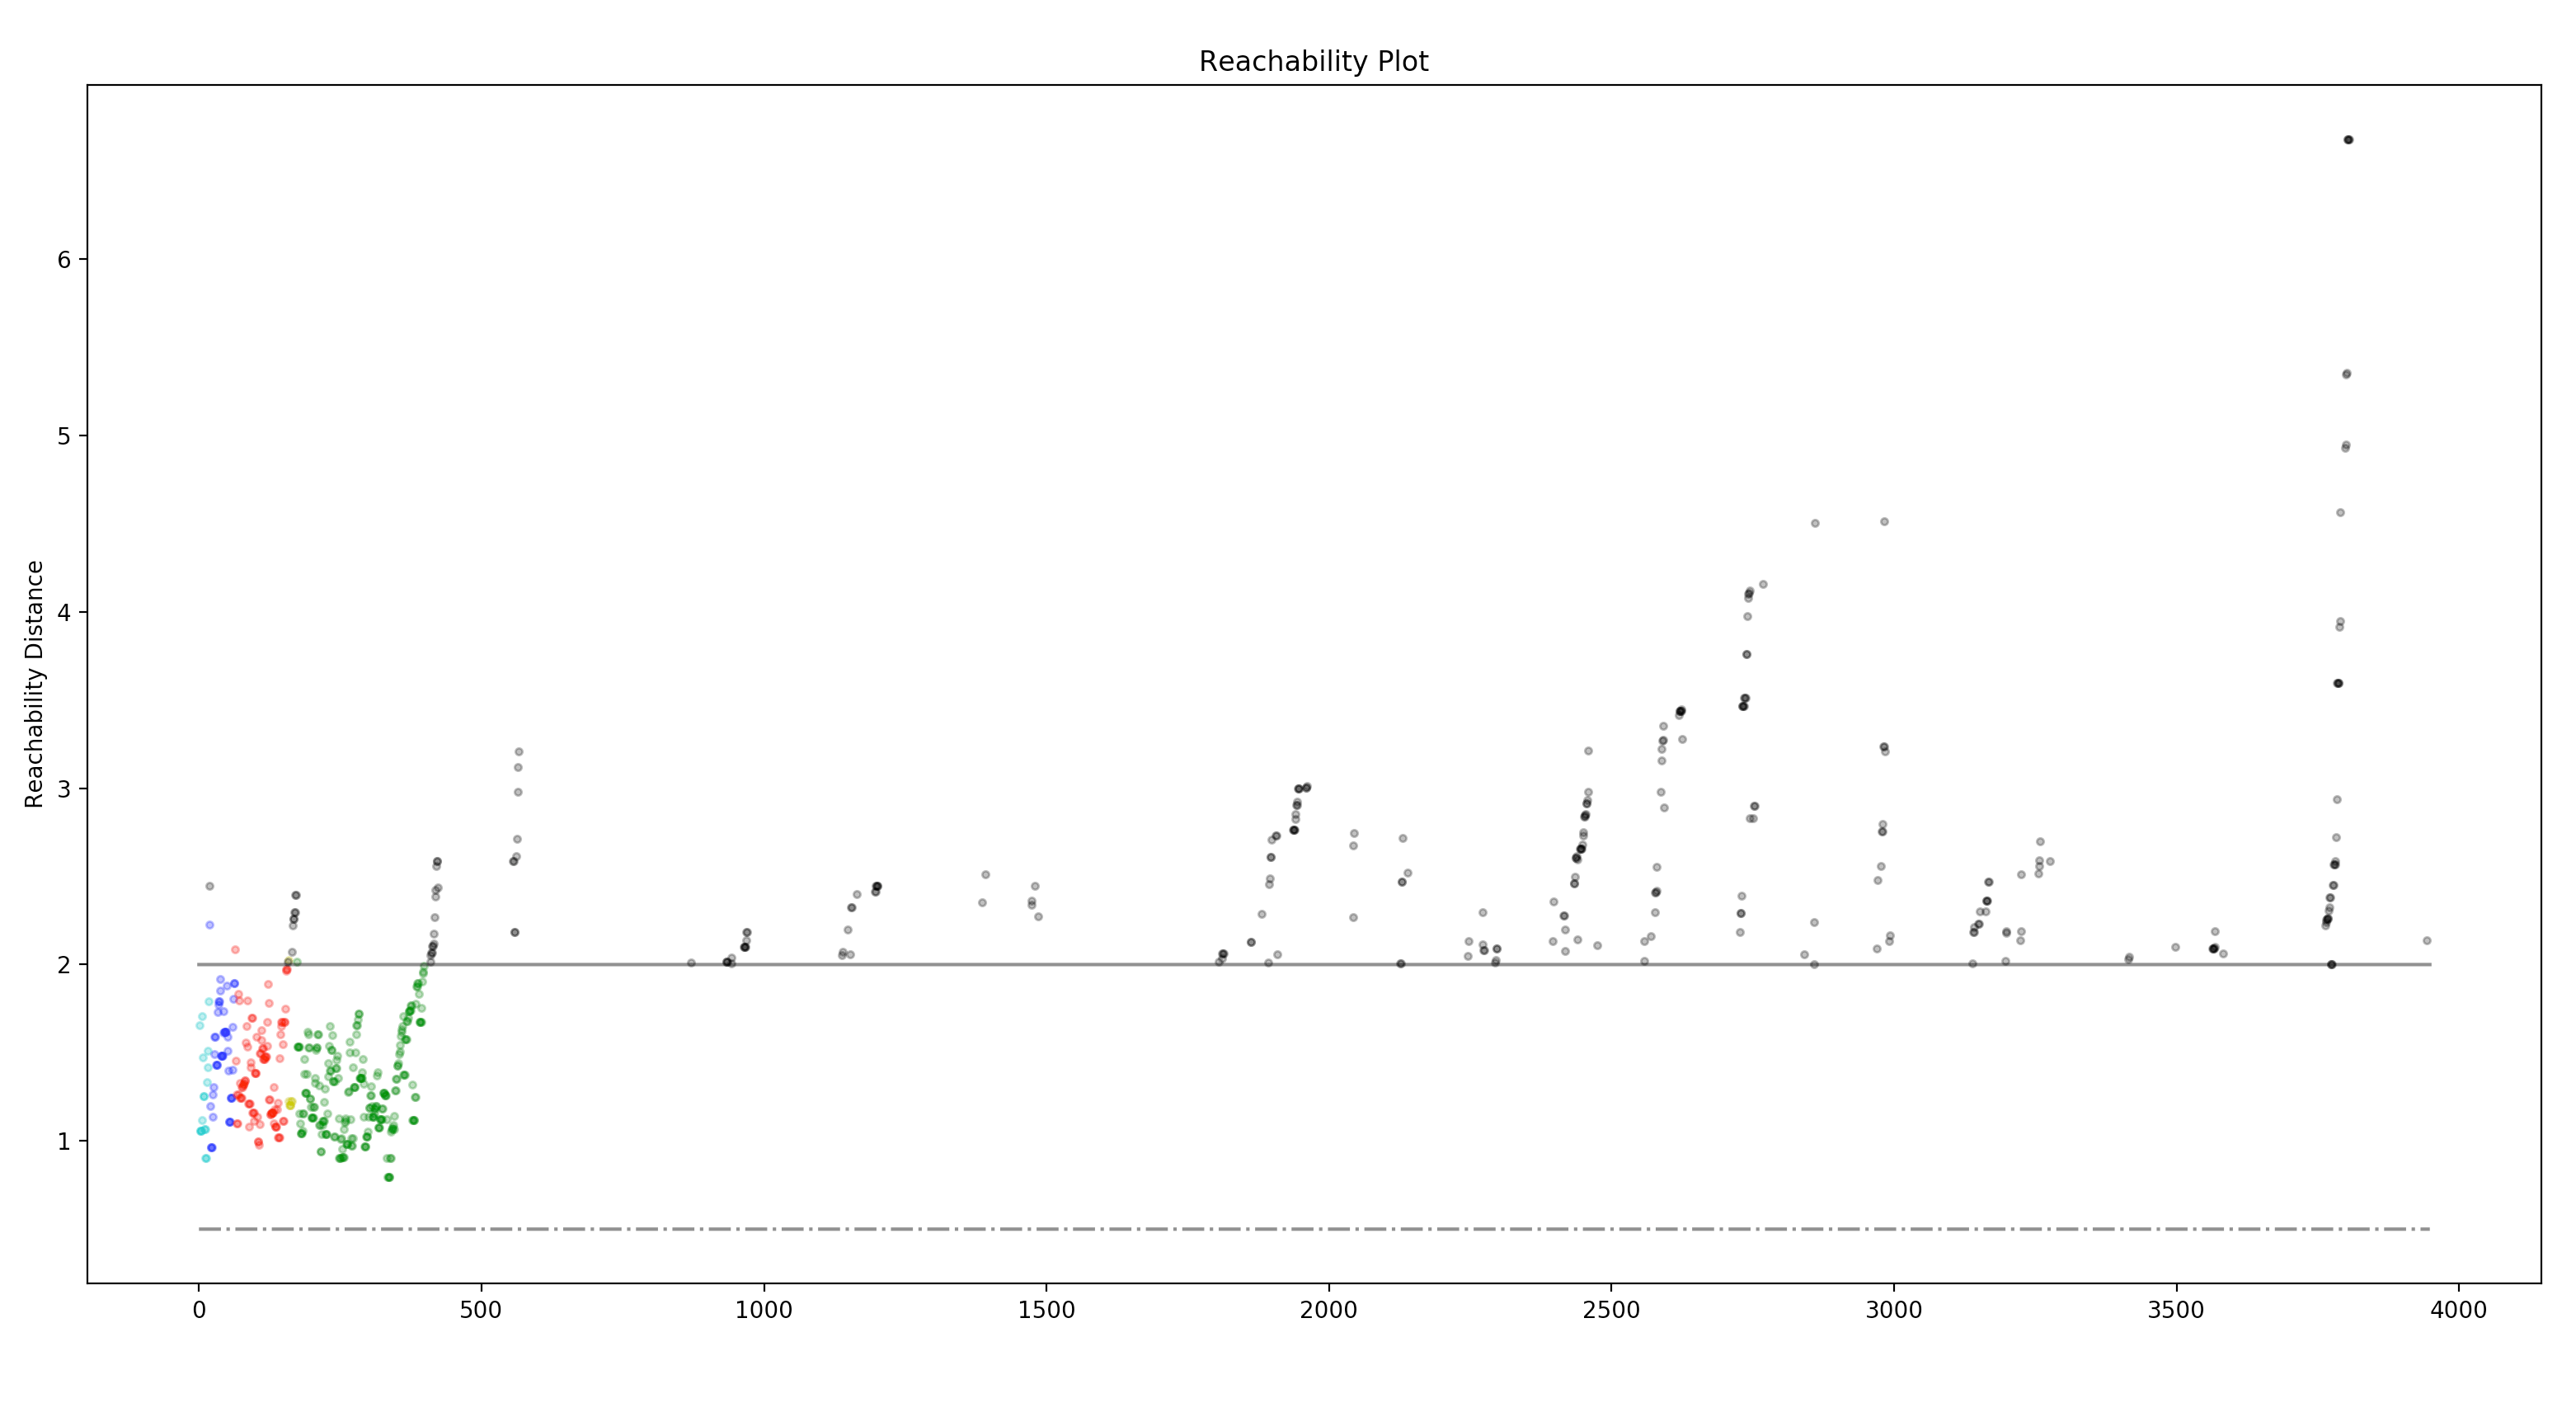
\includegraphics[width=1\textwidth]{./images/clusteringResults/3h-1-reachabilityPlot.png}
    \caption{3h data set OPTICS clustering (first column - 30 min), using DBSCAN clustering.}
    % \label{figure:3h-1-reachabilityPlot}
  \end{subfigure}
  \caption{}
  \label{figure:OPTICSResultsReachabilityPlot}
  \end{figure}

% \begin{figure}[H]
%   \centering
%   \begin{subfigure}{.5\textwidth}
%     \centering
%     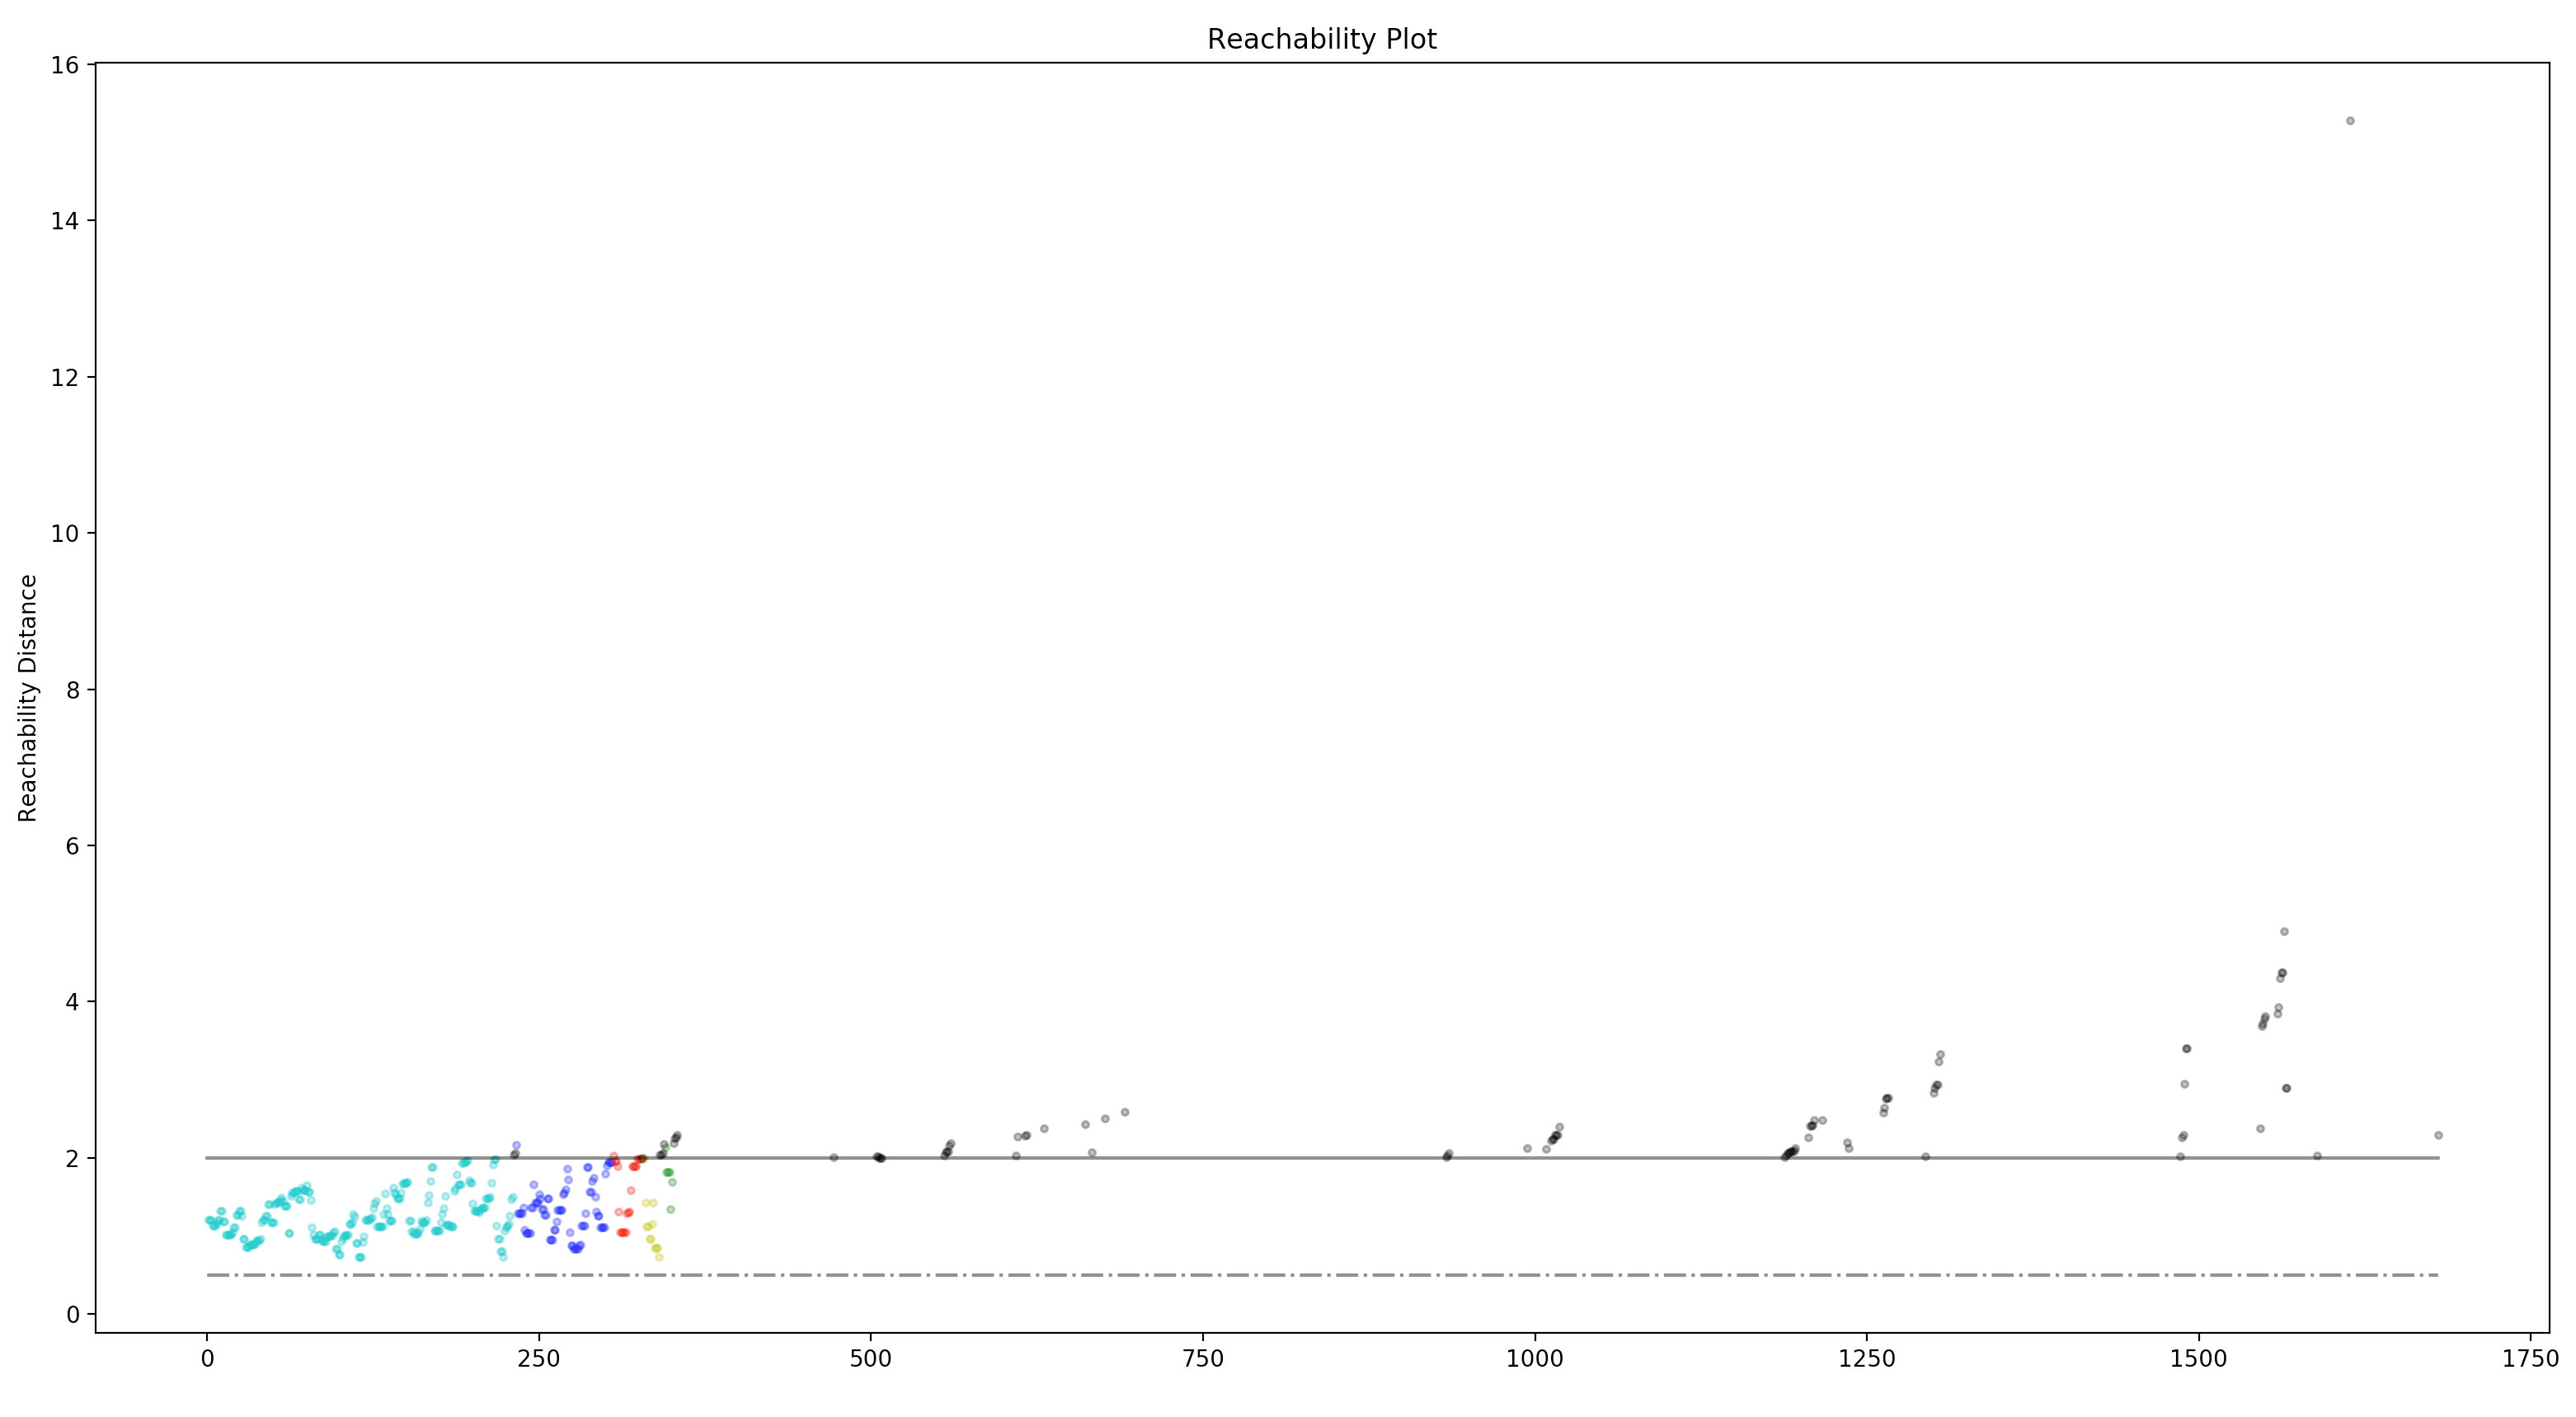
\includegraphics[width=1\textwidth]{./images/clusteringResults/1h-1-reachabilityPlot.png}
%   \caption{}
%   % \label{figure:1h-1-reachabilityPlot}
%   \end{subfigure}%
%   \begin{subfigure}{.5\textwidth}
%     \centering
%     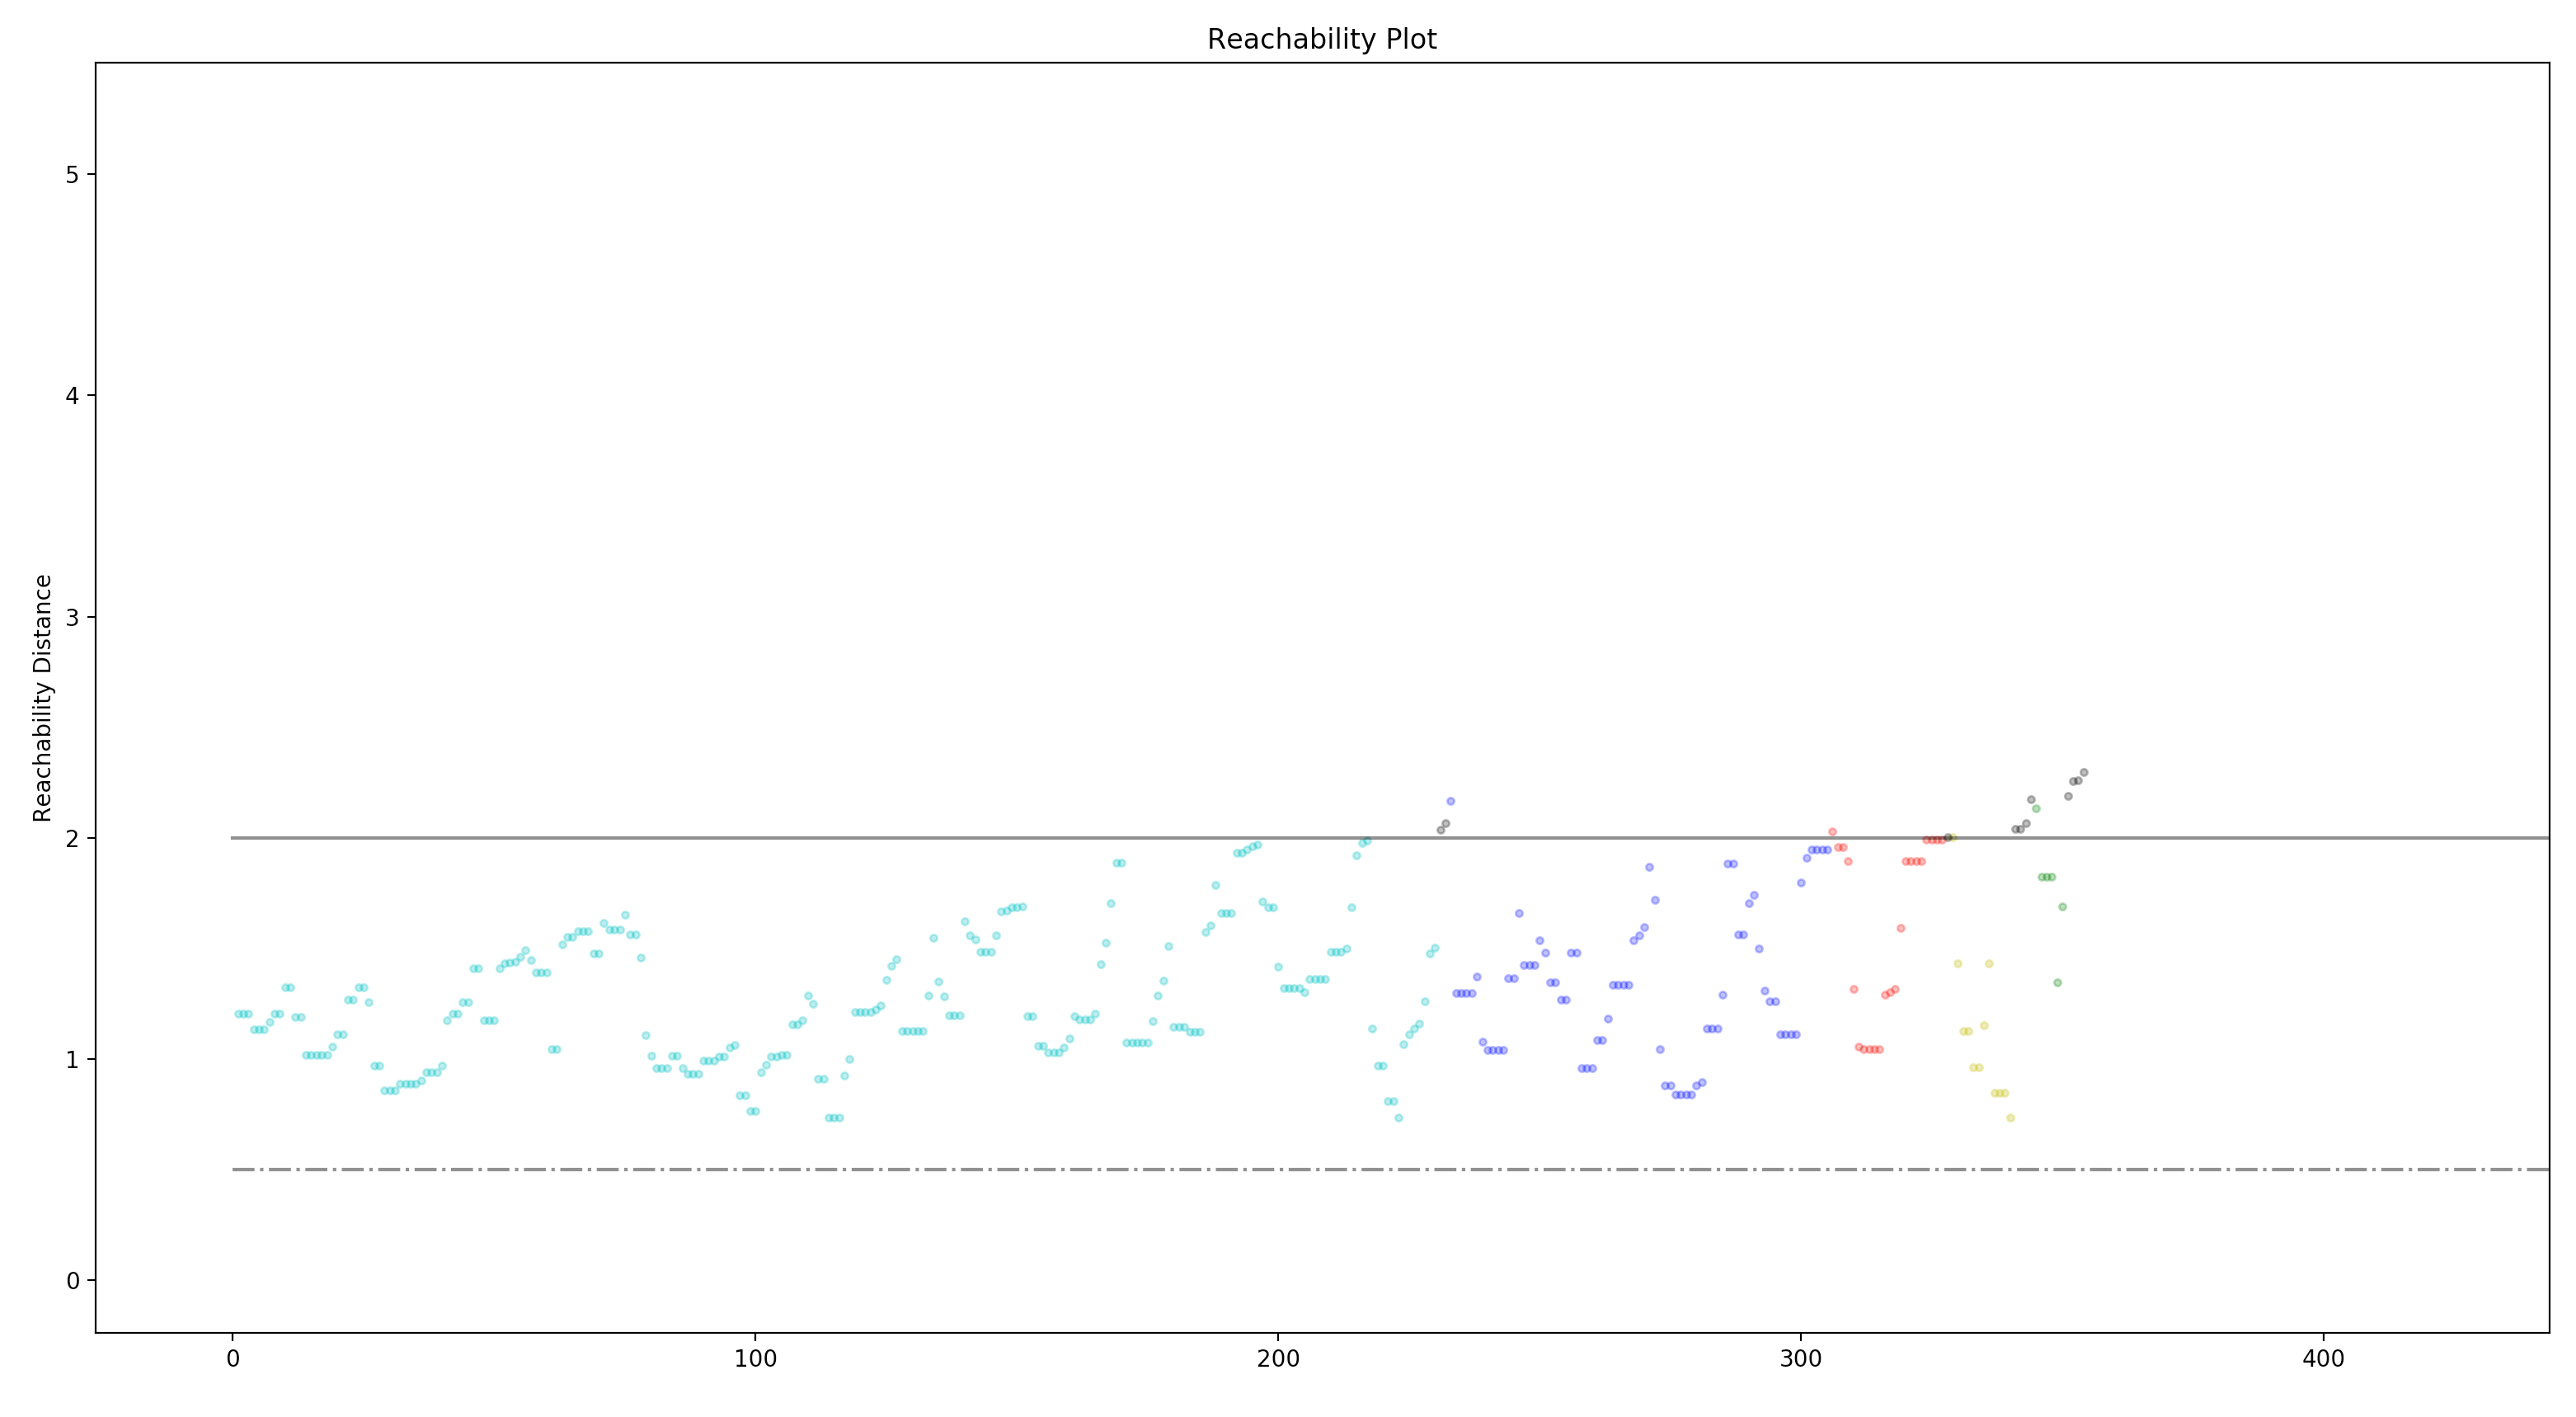
\includegraphics[width=1\textwidth]{./images/clusteringResults/1h-1-reachabilityPlotZoom.png}
%     \caption{}
%     % \label{figure:3h-1-reachabilityPlot}
%   \end{subfigure}
%   \caption{}
%   \label{figure:1h-1-reachabilityPlot}
%   \end{figure}






% optics: two options: xi (automatic technique from \textcite{OPTICS}, or dbscan)





